\documentclass[10pt,a4paper]{article}
\usepackage[latin1]{inputenc}
\usepackage{amsmath}
\usepackage{amsfonts}
\usepackage{amssymb}
\usepackage[dvipsnames,rgb]{xcolor}
\usepackage{graphicx}
\usepackage{listings}
\usepackage[nottoc]{tocbibind}
\author{Baptiste Pauget}
\usepackage[left=2.5cm,right=2.5cm,top=3cm,top=2.5cm]{geometry}
\usepackage{wrapfig}
\usepackage {circuitikz}
\usepackage {tikz}
\usetikzlibrary {positioning}
\usetikzlibrary{intersections}
\usetikzlibrary{calc}
\usepackage{tcolorbox,lipsum}
\usepackage{subfig}
\usepackage{adjustbox}
\usepackage{float}
\usepackage{hyperref}
\hypersetup{
	colorlinks=true,
	linkcolor=blue,
	filecolor=magenta,      
	citecolor=ForestGreen,
	urlcolor=brown,
}
\usetikzlibrary{shapes,snakes}
%\usetikzlibrary{arrows, decorations.markings}

\definecolor {processblue}{rgb}{0.2,0.2,0.96}
\definecolor {processred}{rgb}{0.96,0.2,0.2}
\definecolor {processgreen}{rgb}{0.2,0.96,0.2}
\definecolor {processpurple}{rgb}{0.96,0.2,0.96}
\definecolor {processyellow}{rgb}{0.96,0.96,0.2}
\definecolor {processcyan}{rgb}{0.2,0.96,0.96}
%\definecolor {processred}{HTML}{22F022}
\definecolor {l1}{rgb}{1,1,0}
\definecolor {l2}{rgb}{1,.5,0}
\definecolor {l3}{rgb}{1,0,0}
\definecolor {l4}{rgb}{1,0,1}
\definecolor {l5}{rgb}{0,0,1}



\definecolor {c151515}{HTML}{151515}
\definecolor {cF01515}{HTML}{F01515}
\definecolor {c15F015}{HTML}{15F015}
\definecolor {c1515F0}{HTML}{1515F0}
\definecolor {cF0F015}{HTML}{F0F015}
\definecolor {cF015F0}{HTML}{F015F0}
\definecolor {c15F0F0}{HTML}{15F0F0}
\definecolor {cF0F0F0}{HTML}{F0F0F0}
\definecolor {grey1}{HTML}{D0D0D0}
\definecolor {grey2}{HTML}{E0E0E0}
\definecolor {grey3}{HTML}{F0F0F0}

\newcommand{\code}{\texttt}
\renewcommand{\indent}{~\\\vspace{-.8cm}}
\newcommand{\pindent}{~\\\indent}
\title{\vspace{-1.6cm}M1 Internship : Compiling Whiley to FPGAs}
%
%\tikzstyle{vecArrow} = [thick, decoration={markings,mark=at position
%   1 with {\arrow[semithick]{open triangle 60}}},
%   double distance=1.4pt,
%   preaction = {decorate},
%   postaction = {draw,line width=1.4pt, white}
%   ]

\lstdefinestyle{customc}{
	belowcaptionskip=1\baselineskip,
	breaklines=true,
	frame=single,
	xleftmargin=\parindent,
	showstringspaces=false,
	basicstyle=\small\ttfamily,
	keywordstyle=\bfseries\color{blue!40!black},
	commentstyle=\fontfamily{qcs}\itshape\color{gray!40!black},
	identifierstyle=\color{green!40!black},
	stringstyle=\color{orange},
}

\newcommand{\whileyLine}{\lstinline[language=Whiley,basicstyle=\normalsize\ttfamily]}

\lstdefinelanguage{Whiley}
{
	morekeywords={
		import,
		if,
		else,
		function,
		return,
		int, bool, byte,
		any, void, null,
		ensures,
		requires,
		is,
		all,
		where,
		while,
		type, define, as
	},
	sensitive=true, % keywords are not case-sensitive
	morecomment=[l]{//}, % l is for line comment
	morecomment=[s]{/*}{*/}, % s is for start and end delimiter
	morestring=[b]" % defines that strings are enclosed in double quotes
}

\lstset{
	language	=	Whiley,
	xleftmargin	=	2*\listingnumberwidth,
	numbersep	=	1em,
	captionpos	=	b, % Position of the Caption (t for top, b for bottom)
	extendedchars=	true, % Allows 256 instead of 128 ASCII characters
	tabsize		=	2, % number of spaces indented when discovering a tab 
	columns		=	fixed, % make all characters equal width
	keepspaces	=	true, % does not ignore spaces to fit width, convert tabs to spaces
	showstringspaces=false, % lets spaces in strings appear as real spaces
	breaklines	=	true, % wrap lines if they don't fit
	frame		=	trbl, % draw a frame at the top, right, left and bottom of the listing
%	frameround=tttt, % make the frame round at all four corners
%	framesep=4pt, % quarter circle size of the round corners
	%numbers=left, % show line numbers at the left
	numberstyle	=	\tiny\ttfamily, % style of the line numbers
	commentstyle=	\color{gray}, % style of comments
	%keywordstyle=\color{eclipsePurple}, % style of keywords
	%stringstyle=\color{eclipseBlue}, % style of strings
	%
	numberstyle	=	\small\color{gray},
	%	rulecolor=\color{black},
	keywordstyle=	\color{blue},
	%showlines	=	false,
	style		=	customc
}

\hyphenpenalty=10000


\newcommand{\val}{\mathcal V}
\newcommand{\typ}{\mathcal T}
\newcommand{\ord}{\mathcal O}
\newcommand{\lea}{\mathcal L}


\tikzset{
	-latex, semithick , 
			union/.style ={rectangle, top color = white, bottom color = processblue!20, draw, processblue, text=black, minimum width = 0.6 cm, minimum height = 0.5 cm}, 
			intersection/.style ={rectangle, top color = white, bottom color = processblue!20, draw, processblue, text=black, minimum width = 0.6 cm, minimum height = 0.5 cm}, 
			negation/.style ={rectangle, top color = white, bottom color = processblue!20, draw, processblue, text=black, minimum width = 0.6 cm, minimum height = 0.5 cm}, 
			record/.style ={rectangle, top color = white, bottom color = processblue!20, draw, processblue, text=black, minimum width = 0.6 cm, minimum height = 0.5 cm}, 
			primitive/.style ={rectangle, top color = white, bottom color = processblue!20, draw, processblue, text=black, minimum width = 1.9 cm, minimum height = 0.5 cm, align=center}, 
			leaf/.style ={rectangle, top color = white, bottom color = processred!20, draw, processred, text=black, minimum width = 1.9 cm, minimum height = 0.5 cm, align=center}, 
			root/.style ={rectangle, top color = white, bottom color = processblue!20, draw, processblue, text=black, minimum width = 0.5 cm, minimum height = 0.5 cm, align=center}, 
			general/.style 2 args ={rectangle, top color = white, bottom color = #1!20, draw, #1, text=black, minimum width = #2 cm, minimum height = 0.5 cm, align=center}, 
}


\newcommand{\Dfrac}[2]{%
	\ooalign{%
		$\genfrac{}{}{2.4pt}0{\phantom{#1}}{\phantom{#2}}$\cr%
		$\genfrac{}{}{.8pt}0{#1}{#2}$\cr%
		$\color{white}\genfrac{}{}{.8pt}0{\phantom{#1}}{\phantom{#2}}$}
}



\tikzset{
 shrink inner sep/.code={
   \pgfkeysgetvalue{/pgf/inner xsep}{\currentinnerxsep}
   \pgfkeysgetvalue{/pgf/inner ysep}{\currentinnerysep}
   \pgfkeyssetvalue{/pgf/inner xsep}{\currentinnerxsep - 0.5\pgflinewidth}
   \pgfkeyssetvalue{/pgf/inner ysep}{\currentinnerysep - 0.5\pgflinewidth}
   }
}

\tikzset{horizontal shaded border/.style args={#1 and #2}{
    append after command={
       \pgfextra{%                 
          \begin{pgfinterruptpath}
                \path[rounded corners=2mm,left color=#1,right color=#2]
                ($(\tikzlastnode.south west)+(-\pgflinewidth,-\pgflinewidth)$) 
                rectangle
                ($(\tikzlastnode.north east)+(\pgflinewidth,\pgflinewidth)$);        
           \end{pgfinterruptpath}
        } 
    }
  },
  vertical shaded border/.style args={#1 and #2}{
    append after command={
       \pgfextra{%                 
          \begin{pgfinterruptpath}
                \path[rounded corners,top color=#1,bottom color=#2]
                ($(\tikzlastnode.south west)+(-\pgflinewidth,-\pgflinewidth)$) 
                rectangle
                ($(\tikzlastnode.north east)+(\pgflinewidth,\pgflinewidth)$);        
           \end{pgfinterruptpath}
        } 
    }
  }
}





\pgfdeclareshape{muxB}{
	\anchor{center}{\pgfpointorigin} % within the node, (0,0) is the center
	\anchor{text} % this is used to center the text in the node
	{\pgfpoint{-.5\wd\pgfnodeparttextbox}{-.5\ht\pgfnodeparttextbox}}
	\savedanchor\trueOpt{\pgfpoint{-.6cm}{-.3cm}} % pin 1
	\anchor{in true}{\trueOpt}
	\savedanchor\falseOpt{\pgfpoint{-.6cm}{.3cm}} % pin 2
	\anchor{in false}{\falseOpt}
	\savedanchor\cond{\pgfpoint{0cm}{-.8cm}} % pin 3
	\anchor{in cond}{\cond}
	\savedanchor\res{\pgfpoint{.6cm}{.0cm}} % pin 3
	\anchor{out}{\res}
	\foregroundpath{ % border and pin numbers are drawn here
		\pgfsetlinewidth{0.03cm}
		\pgfplothandlerpolygon
		\pgfplotstreamstart
		\pgfplotstreampoint{\pgfpoint{-.3cm}{-.6cm}}
		\pgfplotstreampoint{\pgfpoint{.3cm}{-.4cm}}
		\pgfplotstreampoint{\pgfpoint{.3cm}{.4cm}}
		\pgfplotstreampoint{\pgfpoint{-.3cm}{.6cm}}
		\pgfplotstreamend
		\pgfusepath{draw} 
		\pgfsetlinewidth{0.02cm}
		\pgfpathmoveto{\pgfpoint{-.3cm}{.3cm}}
		\pgfpathlineto{\pgfpoint{-.6cm}{.3cm}}
		\pgfpathmoveto{\pgfpoint{-.3cm}{-.3cm}}
		\pgfpathlineto{\pgfpoint{-.6cm}{-.3cm}}
		\pgfpathmoveto{\pgfpoint{.3cm}{0cm}}
		\pgfpathlineto{\pgfpoint{.6cm}{0cm}}
		\pgfpathmoveto{\pgfpoint{0cm}{-.5cm}}
		\pgfpathlineto{\pgfpoint{0cm}{-.8cm}}
		\pgftext[left,at={\pgfpoint{-.2cm}{.3cm}}]{\scriptsize {$0$}}
		\pgftext[left,at={\pgfpoint{-.2cm}{-.3cm}}]{\scriptsize {$1$}}
		\pgfusepath{draw}
}}

\pgfdeclareshape{muxT}{
	\anchor{center}{\pgfpointorigin} % within the node, (0,0) is the center
	\anchor{text} % this is used to center the text in the node
	{\pgfpoint{-.5\wd\pgfnodeparttextbox}{-.5\ht\pgfnodeparttextbox}}
	\savedanchor\trueOpt{\pgfpoint{-.6cm}{.3cm}} % pin 1
	\anchor{in true}{\trueOpt}
	\savedanchor\falseOpt{\pgfpoint{-.6cm}{-.3cm}} % pin 2
	\anchor{in false}{\falseOpt}
	\savedanchor\cond{\pgfpoint{0cm}{.8cm}} % pin 3
	\anchor{in cond}{\cond}
	\savedanchor\res{\pgfpoint{.6cm}{.0cm}} % pin 3
	\anchor{out}{\res}
	\foregroundpath{ % border and pin numbers are drawn here
		\pgfsetlinewidth{0.03cm}
		\pgfplothandlerpolygon
		\pgfplotstreamstart
		\pgfplotstreampoint{\pgfpoint{-.3cm}{-.6cm}}
		\pgfplotstreampoint{\pgfpoint{.3cm}{-.4cm}}
		\pgfplotstreampoint{\pgfpoint{.3cm}{.4cm}}
		\pgfplotstreampoint{\pgfpoint{-.3cm}{.6cm}}
		\pgfplotstreamend
		\pgfusepath{draw} 
		\pgfsetlinewidth{0.02cm}
		\pgfpathmoveto{\pgfpoint{-.3cm}{.3cm}}
		\pgfpathlineto{\pgfpoint{-.6cm}{.3cm}}
		\pgfpathmoveto{\pgfpoint{-.3cm}{-.3cm}}
		\pgfpathlineto{\pgfpoint{-.6cm}{-.3cm}}
		\pgfpathmoveto{\pgfpoint{.3cm}{0cm}}
		\pgfpathlineto{\pgfpoint{.6cm}{0cm}}
		\pgfpathmoveto{\pgfpoint{0cm}{.5cm}}
		\pgfpathlineto{\pgfpoint{0cm}{.8cm}}
		
		\pgftext[left,at={\pgfpoint{-.2cm}{.3cm}}]{\scriptsize {$1$}}
		\pgftext[left,at={\pgfpoint{-.2cm}{-.3cm}}]{\scriptsize {$0$}}
		\pgfusepath{draw}
}}
\pgfdeclareshape{Block}{
	\anchor{center}{\pgfpointorigin} % within the node, (0,0) is the center
	\anchor{text} % this is used to center the text in the node
	{\pgfpoint{-.5\wd\pgfnodeparttextbox}{-.5\ht\pgfnodeparttextbox}}
	\savedanchor\a{\pgfpoint{-1.8cm}{.55cm}} % pin 1
	\anchor{in start}{\a}
	\savedanchor\b{\pgfpoint{-1.8cm}{-.55cm}} % pin 2
	\anchor{in data}{\b}
	\savedanchor\c{\pgfpoint{1.8cm}{.55cm}} % pin 3
	\anchor{out done}{\c}
	\savedanchor\d{\pgfpoint{1.8cm}{-.55cm}} % pin 3
	\anchor{out data}{\d}
	\foregroundpath{ % border and pin numbers are drawn here
		\pgfsetlinewidth{0.03cm}
		\pgfpathrectanglecorners{\pgfpoint{1.5cm}{1cm}}{\pgfpoint{-1.5cm}{-1cm}}
		\pgfusepath{draw} 
		\pgfsetlinewidth{0.02cm}
		\pgfpathmoveto{\pgfpoint{-1.5cm}{.55cm}}
		\pgfpathlineto{\pgfpoint{-1.8cm}{.55cm}}
		\pgfpathmoveto{\pgfpoint{-1.5cm}{-.55cm}}
		\pgfpathlineto{\pgfpoint{-1.8cm}{-.55cm}}
		\pgfpathmoveto{\pgfpoint{1.5cm}{.55cm}}
		\pgfpathlineto{\pgfpoint{1.8cm}{.55cm}}
		\pgfpathmoveto{\pgfpoint{1.5cm}{-.55cm}}
		\pgfpathlineto{\pgfpoint{1.8cm}{-.55cm}}
		
		\pgftext[left,at={\pgfpoint{-1.4cm}{.55cm}}]{\scriptsize {Start}}
		\pgftext[left,at={\pgfpoint{-1.4cm}{-.55cm}}]{\scriptsize {Data}}
		\pgftext[right,at={\pgfpoint{1.4cm}{.55cm}}]{\scriptsize {Done}}
		\pgftext[right,at={\pgfpoint{1.4cm}{-.55cm}}]{\scriptsize {Data}}
		
		\pgfusepath{draw}
}}
\pgfdeclareshape{BlockCB}{
	\anchor{center}{\pgfpointorigin} % within the node, (0,0) is the center
	\anchor{text} % this is used to center the text in the node
	{\pgfpoint{-.5\wd\pgfnodeparttextbox}{-.5\ht\pgfnodeparttextbox}}
	\savedanchor\a{\pgfpoint{-2.3cm}{1.1cm}} % pin 1
	\anchor{in start}{\a}
	\savedanchor\b{\pgfpoint{-2.3cm}{-1.1cm}} % pin 2
	\anchor{in data}{\b}
	\savedanchor\c{\pgfpoint{2.3cm}{1.1cm}} % pin 3
	\anchor{out done}{\c}
	\savedanchor\d{\pgfpoint{2.3cm}{-1.1cm}} % pin 3
	\anchor{out data}{\d}
	\savedanchor\e{\pgfpoint{2.3cm}{0cm}} % pin 3
	\anchor{out test}{\e}
	\foregroundpath{ % border and pin numbers are drawn here
		\pgfsetlinewidth{0.03cm}
		\pgfpathrectanglecorners{\pgfpoint{2cm}{1.5cm}}{\pgfpoint{-2cm}{-1.5cm}}
		\pgfusepath{draw} 
		\pgfsetlinewidth{0.02cm}
		\pgfpathmoveto{\pgfpoint{-2cm}{1.1cm}}
		\pgfpathlineto{\pgfpoint{-2.3cm}{1.1cm}}
		\pgfpathmoveto{\pgfpoint{-2cm}{-1.1cm}}
		\pgfpathlineto{\pgfpoint{-2.3cm}{-1.1cm}}
		\pgfpathmoveto{\pgfpoint{2cm}{1.1cm}}
		\pgfpathlineto{\pgfpoint{2.3cm}{1.1cm}}
		\pgfpathmoveto{\pgfpoint{2cm}{0cm}}
		\pgfpathlineto{\pgfpoint{2.3cm}{0cm}}
		\pgfpathmoveto{\pgfpoint{2cm}{-1.1cm}}
		\pgfpathlineto{\pgfpoint{2.3cm}{-1.1cm}}
		
		\pgftext[left,at={\pgfpoint{-1.9cm}{1.1cm}}]{\scriptsize {Start}}
		\pgftext[left,at={\pgfpoint{-1.9cm}{-1.1cm}}]{\scriptsize {Data}}
		\pgftext[right,at={\pgfpoint{1.9cm}{1.1cm}}]{\scriptsize {Done}}
		\pgftext[right,at={\pgfpoint{1.9cm}{0cm}}]{\scriptsize {Test}}
		\pgftext[right,at={\pgfpoint{1.9cm}{-1.1cm}}]{\scriptsize {Data}}
		
		\pgfusepath{draw}
}}

\pgfdeclareshape{Reg}{
	\anchor{center}{\pgfpointorigin} % within the node, (0,0) is the center
	\anchor{text} % this is used to center the text in the node
	{\pgfpoint{-.5\wd\pgfnodeparttextbox}{-.5\ht\pgfnodeparttextbox}}
	\savedanchor\a{\pgfpoint{.5cm}{0cm}} % pin 1
	\anchor{east}{\a}
	\savedanchor\b{\pgfpoint{-.5cm}{0cm}} % pin 2
	\anchor{west}{\b}
	\savedanchor\c{\pgfpoint{0cm}{.5cm}} % pin 3
	\anchor{north}{\c}
	\savedanchor\d{\pgfpoint{0cm}{-.5cm}} % pin 3
	\anchor{south}{\d}
	\foregroundpath{ % border and pin numbers are drawn here
		\pgfsetlinewidth{0.03cm}
		\pgfpathrectanglecorners{\pgfpoint{.5cm}{.5cm}}{\pgfpoint{-.5cm}{-.5cm}}
		\pgfusepath{draw} 
		\pgfsetlinewidth{0.01cm}
		\pgfpathmoveto{\pgfpoint{-.5cm}{0cm}}
		\pgfpathlineto{\pgfpoint{0cm}{.5cm}}
		\pgfpathmoveto{\pgfpoint{-.5cm}{-.5cm}}
		\pgfpathlineto{\pgfpoint{.5cm}{.5cm}}
		\pgfpathmoveto{\pgfpoint{0cm}{-.5cm}}
		\pgfpathlineto{\pgfpoint{.5cm}{0cm}}
		
		\pgftext[center,at={\pgfpoint{0cm}{0cm}}]{\textbf{Reg}}
		
		\pgfusepath{draw}
}}




\begin{document}
	
	\setcounter{tocdepth}{2}
\maketitle
\section*{Introduction}\indent
\addcontentsline{toc}{section}{Introduction}

Improving code performances lies more and more in the relevant use of computational helpers \cite{nikolov2008systematic}. Computing platforms like OpenCL or CUDA that enable to relocate resource consuming calculations to graphics processing unit (GPU) are now ordinary. Theses frameworks are rather low-level and require either a thorough learning or the use of higher level libraries that reduce their flexibility. A orthogonal concern of programming language is static checking. As the rise of strongly typed languages (Rust, Scala, Haskell, ...) reveals it, extended static checking is well-liked since it improves greatly the development process, lowering the debug work \cite{flanagan2013pldi}. 
The Whiley language goes a step further, by providing an embedded support for specification, giving a chance to adjust the scope of compilation-time checks. Targeting Field Programmable Gate Arrays (FPGAs) for Whiley compilation tries to reconcile this two goals.


\section*{Acknowledgements}\indent

I would like to thank D. J. Pearce and A. Potanin for welcoming me in the Programming Languages Research group of Victoria University of Wellington and helping me during this internship. 

Thanks a lot to T. Bourke, M. Pouzet and I. Delais without whom I could not have come to Wellington.

\tableofcontents


\newpage

\section{Working with FPGAs}\indent

Field Programmable Gate Arrays (FPGAs) are integrated circuits that can be configure by the user without any knowledge in electronics. Their use nevertheless requires a specific work-flow that needs to be understood to write relevant FPGA configurations.


\subsection{A specific hardware} \indent

FPGAs try to gather the power of Application Specific Integrated Circuits (ASICs) with the flexibility of general computation devices (CPUs), by giving a way to reconfigure hardware without any physical operations.

\subsubsection{Usage}
\indent

FPGA's behaviour is defined by loading a hardware configuration at its start-up. Inputs and outputs of the device can then be used in a wider system as if they were separated by the requested circuit. This flexibility makes them appropriated for

\begin{itemize}
	\item \textbf{Prototyping ASICs} : ASICs are still faster than FPGAs but they cannot be reconfigured once they are built. FPGAs allow their development process to be easier and cheaper.
	\item \textbf{Computation helpers} : The performance of specific applications (e.g., images processing, etc) can be enhanced with hardware compiled functions (e.g., Fast Fourier Transform), that are intensively used (FPGAs are often part of supercomputers).
	\item \textbf{Highly parallel applications} : because of their high parallelism potential, FPGAs are useful in applications that process lots of data simultaneously, like network interfaces (where large bandwidth is needed).
\end{itemize}



\begin{wrapfigure}[18]{r}{.4\textwidth}
	\vspace{-60pt}
	\center
	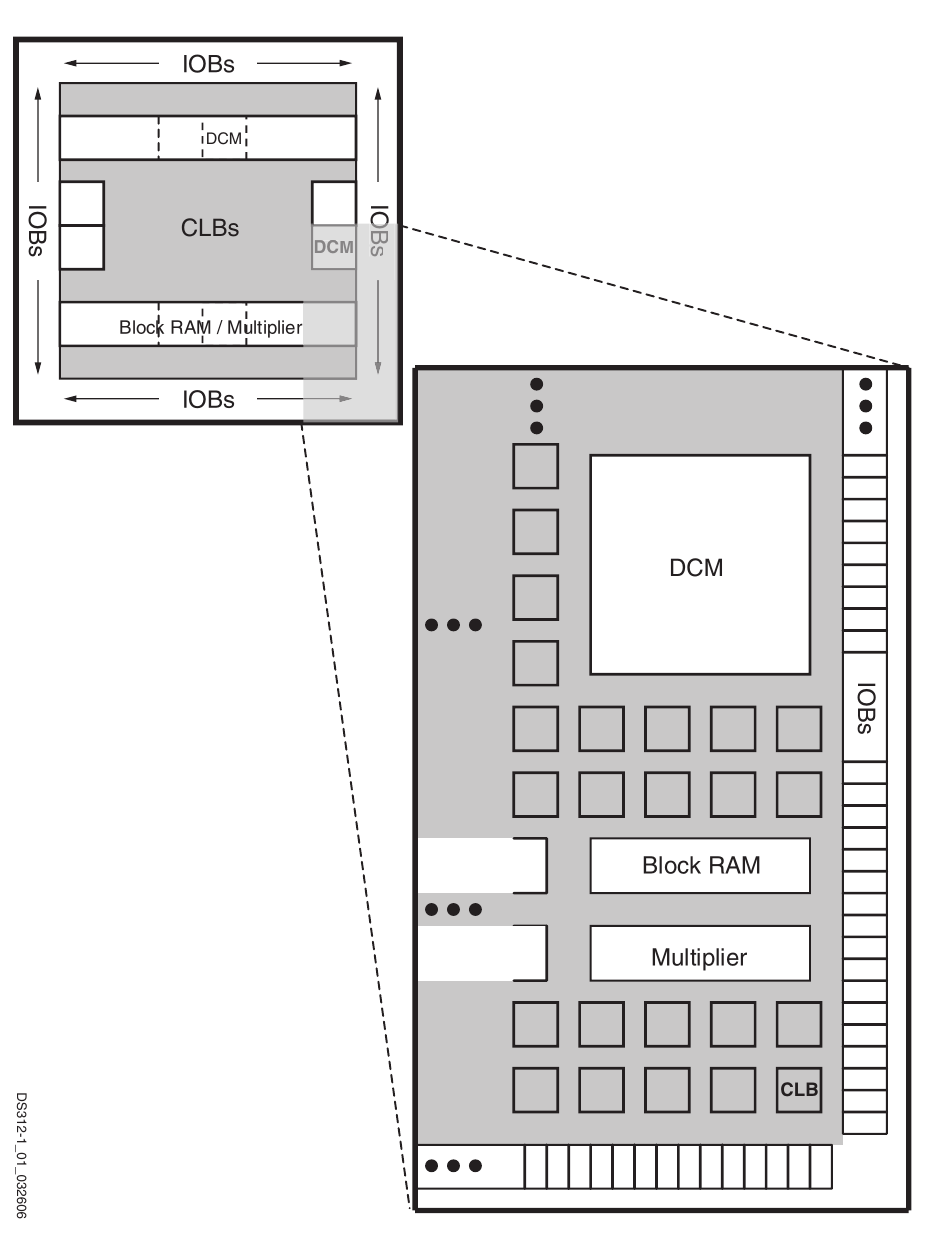
\includegraphics[scale=0.26]{Spartan.png}
	\caption{Spartan-3A Architecture \cite{Spartan}}
	\label{Sptan3A}
\end{wrapfigure}

\subsubsection{Structural organisation}\indent

FPGAs are organised as an array of interconnected identical computation cells, fortified with specific circuits. The coarse structure of FPGAs is illustrated in \autoref{Sptan3A} and contains the following components (with their number in Spartan XC3S500E devices) :

\begin{itemize}
	\item \textbf{Configurable Logic Blocks (CLB)} (1,164) : The atomic units of FPGAs.
	They are divided in four slices  containing
	\begin{itemize}
		\item \textbf{2 Look-Up Tables} (LUT) : Implementation of logic computation in small LUTs (4 to 1 bits) that enable to compute any boolean function (They are RAM memory based)
		\item \textbf{2 Storage Elements} : Can be used as flip-flops (registers) or latches
	\end{itemize}
	\item \textbf{Input/Outputs Blocks} (232) : They provide an interface to the outside, preserving the internal impedances used in the FPGA.
\end{itemize}

\begin{itemize}
	\item \textbf{RAM Blocks} (20 : 368,640 bits) : These 18Kbits blocks can be used as RAM/ROM, with one or two I/O ports, supporting several memory configurations. (reading or writing up to 36 bits on each port).
	\item \textbf{Multipliers Blocks} (20) : They avoid an overuse of CLBs for multiplicative operations.
	\item \textbf{Digital Clock Manager Blocks} : They can duplicate, multiply, divide and delay clock signals
\end{itemize}

Some additional specific logic is provided to improve performances for complex operations (carry/arithmetic logic, dedicated multiplexers, ...).




\subsection{Hardware Description Languages - VHDL}
\indent

The lowest level description of FPGA's configurations is net-lists, which represents components and connexions between them. Higher-level descriptions were developed including circuit diagrams and hardware description languages (HDLs). The most used ones are Verilog and VHDL. Because of available documentation and a seemingly easier learning curve than Verilog, VHDL was chosen as the targeted language of the compiler developed during this project. A brief introduction to the main aspects of this language follows\cite{FRV}.



\begin{wrapfigure}[16]{r}{.48\textwidth}
	\vspace{-35pt}
\begin{lstlisting}[language=VHDL]
library ieee;
use ieee.std_logic_1164.all;
use ieee.numeric_std.all;
	
entity foo is
  port (
    foo_in  : in  signed(31 downto 0);
    foo_out : out signed(31 downto 0)
  );
end entity foo;
	
architecture Behavioural of foo is
  -- Declarations
begin
 -- Circuit description
end architecture Behavioural;
\end{lstlisting}
\label{VHDL}
\end{wrapfigure}

\subsubsection{Overview}\indent

Contrary to Verilog, VHDL (VHSIC Hardware Description Language) is a typed HDL: wires or bench of wires are represented with typed \textit{signals} and the correctness of statements is checked during compilation.\\

As in numerous programming languages, sources are structured in packages and libraries.
The main compilation unit is the \textbf{entity}, that defines an interface (input/output signals) and comes with one or more \textbf{architectures} that describe the inner circuit.


\subsubsection{Describing the circuit} \indent

VHDL is a data-flow language: a signal represents the state of some data at a precise place of the computation and architecture statements depict operations that link these signals. Their order is thus insignificant and signals can be assigned at most once.


\paragraph{Concurrent statements: the combinatorial description} \pindent
\label{Concurr}

A combinatorial circuit does not contain any loop. This ensure that it will stabilize if the inputs keep their values a long enough time. The following concurrent statements are converted to combinatorial circuits during the compilation of VHDL toward an FPGA configuration file.

\begin{itemize}
	\item \textbf{Signal assignments} (\code{<=}) that link the result of an expression to a signal. Expressions are defined using signals and bitwise operations or typed operations whose circuit are described in imported libraries (addition, multiplication, ...).
	\item \textbf{Conditional signal assignments} (\code{when}/\code{select}) that construct multiplexers choosing between several signals by examining the values of other ones.
	\item \textbf{Component instantiations} that instantiate external entities, linking their interface with internal signals. They correspond to software programming languages' function call except in the fact that the circuit is duplicated at each instantiation.
	\item \textbf{Process statements} that introduce an other kind of description of circuit discussed below.
\end{itemize}


\paragraph{Sequential statements : the behavioural description}\pindent

Process statements delineated a description that is closer to software programming languages: its inner statements are executed sequentially and higher level constructions such as variables or \code{if} statements are available. Variables strongly differ from signals in that they are accessible inside the \code{process} statement only, and they behave as software programming languages' variables, holding the last assigned value. More work is done by the compiler to convert these statements to a circuit that will behave as described. It results in a larger configuration and a longer compilation time.

\subsubsection{Execution model}

\paragraph{Parallelism}\pindent


Concurrent statements are independently re-evaluated when an event occurs on one of their signals they are sensitive to. This sensitivity list is implicitly set to the read signals of the expression except for \code {process} statements that defines it explicitly. The completion of expression's evaluation triggers a event on the signals that are written by it.\\

Concurrent statements are atomic computation units : every outputs are set at the same time. This is particularly important for \code {process} statements : read signals hold the value they had at the start of the evaluation, and the ones that are written are all updated at the same time at the end of the process. A signal that is writen several time through the process will only keep the last value.

\paragraph{Considerations on time}\pindent


The evaluation of expressions is completed when circuit's output impedances are stabilized, after a change in its inputs. The laws of physics prevent it to be immediate, and the require time is known as \textit{delta-delay}. These delays should not interfere with the design conception, but may prevent result to comply with frequency constraints.\\

Introducing time in a design is achieved with external clocks. Usual boards that contain FPGAs include several clocks connected with predefined input ports. Using specific clock manager blocks, these signals can be duplicated and their frequency changed. 
To ensure the configuration will behave the desired way, clock's frequencies must be low enough to ensure that the period is greater than the \textit{delta-delay} of the clocked circuit. 

	\begin{wrapfigure}[7]{r}{.2\textwidth}
	\vspace{-40pt}
		\center
		\begin{circuitikz}[scale=.7, transform shape, -,terminal/.style={
				% The shape:
				rounded rectangle,
				minimum size=1.6mm,
				% The rest
				thick,draw=black}]
			
			\draw (0, 1) node[nor port] (S) {};
			\draw (S)+(-.56,0) node {Nor};
			\draw (0,-1) node[nor port] (R) {};
			\draw (R)+(-.56,0) node {Nor};
			\draw (S.out) -- ++(0,-.5) -- ($(R.in 1)+(0,.5)$) -- (R.in 1);
			\draw (R.out) -- ++(0,.5) -- ($(S.in 2)+(0,-.5)$) -- (S.in 2);
		
		\node at ($(S.in 1)-(.8,0)$) (s) {\huge s};
		\draw (s) --  (S.in 1);
		\node at ($(R.in 2)-(.8,0)$) (r) {\huge r};
		\draw (r) --  (R.in 2);
		\node at ($(R.out)+(.8,0)$) (x) {\huge x};
		\draw (x) --  (R.out);
			
		\end{circuitikz}
		\caption{SR-latch}
		\label{FlFl}
		\label{Dloops}
	\end{wrapfigure}


\subsubsection{Registers}\indent


Storing values between updating orders is a very useful feature that is usually achieved using \textit{latches} or \textit{flip-flops}. \autoref{FlFl} shows the circuit of a set-reset latch. This circuits are intended to be used with at most one active input and are non-combinatorial since they contain feed-backs : their outputs depend indirectly of themselves. Such feed-backs are called \textit{positive} when the circuit can become stabilized and \textit{latches} or \textit{flip-flops} are of this kind. \\


\begin{wrapfigure}[8]{r}{.32\textwidth}
	\vspace{-15pt}
\begin{lstlisting}[language=VHDL, frame=single, title=Register generation]
Reg: process(clock) is
begin
  if (rising_edge(clock)) then
    reg <= newValue;
  end if;
end process Reg;
\end{lstlisting}
\end{wrapfigure}

Registers are signals that update their value only when an event occurs on other one. They are mainly used with a clock signal as trigger. They are inferred by the synthesizer when an incomplete if statements is encountered in a process statement: \code{if} a signal is set in only some branches of a disjunction, a register will be generated. To avoid unwanted effects, \code{if} statements have to be carefully used.





\subsection{The compilation process} \indent

The compilation of VHDL code to an FPGA configuration file is a complex and time consuming process. Sources are first converted to net-lists (the synthesis) that are used to generate the configuration. 

\subsubsection{Compilation step} \indent

The compilation of net-lists to a configuration file strongly depends on the targeted device and is handled by commercial tools provided by FPGAs vendors.  The major steps of the this process are :

\begin{itemize}
	\item \textbf{Mapping} : Conversion of net-list operations to LUTs and specific logic blocks that are available on the device.
	\item \textbf{Place and route} : Positioning the LUTs and specific blocks on the FPGA, regarding the constraints (output pins, clocks), and drawing the connections between theses blocks.
	\item \textbf{Time analysis} : Analysis of the circuit to determine the maximum delay needed for it to get stabilized on a change of its inputs.
	\item \textbf{Configuration generation} : Generating a configuration file that can be loaded on the FPGA.
\end{itemize}


\subsubsection{Simulations} \indent

Because of the expensive time cost of synthesis (about 1 minute 30 seconds for simple VHDL sources) and the poor debugging aids on FPGAs, simulators provide a way to enhance the development process. Simulations can be run at several steps in the compilation process.
They enable one to investigate configuration's behaviour in an almost interactive way, giving access to inner signal impedances, and their evolution through time.\\

Simulations are supported inside VHDL, with special statements (like \lstinline[language=VHDL,basicstyle=\ttfamily\normalsize]{wait for 2ms}), operations or data types (floats) that are not supported by the synthesizer but that make the analysis easier. Values of inputs signals of the studied entity are planned with a separated VHDL file.





\subsection{Existing high level compilers} \indent

To bridge the gap between hardware and software programming and make the use of FPGAs accessible for non-specialists, high-level compilers have been developed that compile software programming languages to HDL descriptions \cite{bacon2013fpga} or net-lists \cite{iseli1995c++}.

\subsubsection{Targeted execution environments} \indent

Most of the high-level compilation tools target highly heterogeneous systems, aiming at providing a unique language to describe both software and hardware parts. These execution environments can be composed of multiple CPUs, GPUs, FPGAs or other specific hardware devices.\\

Theses systems are often built around a main processor that organises the computation on helpers. OpenCL provides unified abstractions to program highly parallel applications, and have been adapted to target FPGAs \cite{czajkowski2012opencl}.


\subsubsection{Xilinx's Vivado tool} \indent

The Vivado Design Suite gathers tools to develop software applications with hardware parts. A C to HDL compiler is included that enables hardware to be described in C. The supported language is relatively wide and includes general loops that are converted to complex state machines. Because these hardware circuits are intended to be part of a larger system, they are constructed with additional interface signals for linking components together (\code {start}, \code {done}, \code {ready} and \code {idle} signals). 


\subsubsection{Limitation} \indent

In several high level compiler studies, the supported language was restricted to a very small and basic core of the original language. Process statements were used to convert easily basic C code to VHDL \cite{parkinson1994c} but such solutions only bridge the (huge) syntactical gap between C and VHDL, providing no more abstractions that VHDL ones.\\


Most of chosen source languages were deeply imperative languages (C, Java) that increases a lot the conceptual gap between hardware descriptions and them. Using more functional languages could give a more accurate high-level description. [TODO asynchronous languages ?]\\

High level compilers also tried to add as few elements as possible in the source language. The compiler then adds a lot of VHDL elements and this gives few ways to control precisely  the produced code. Modifying the source language by providing meaningful syntax constructions could make it a true high-level hardware description language, more than a software programming language with a tool that obscurely converts it to a hardware description.


\section{The Whiley language and the compiler framework}
\indent

The Whiley language is designed to provide extended static checking. The strong type system is coupled with support for specification that can be verified by a theorem prover.\\ 

The following presentation of the Whiley language focuses on the aspects that were studied in this work, that is especially unrelated to the specification and checking parts of the language. An exhaustive documentation can be found \href{http://www.whiley.org/}{here} \cite{WhileySpec}.


\subsection{Overview}\indent

With a Python like syntax (with C-like comments), Whiley is both
\begin{itemize}
\item Oriented-object : Records and open records enable to define values with attributes and methods.
\item Functional : First class functions are provided : functions (pure) or methods (can have side effects) can be used as values.
\end{itemize}

Specification is introduced through the \whileyLine{requires}, \whileyLine{ensures} and \whileyLine{where} keywords. Here is a typical Whiley program that illustrates how to build a specified function.

\begin{lstlisting}[language=Whiley,numbers=left]
function firstIndexOf(int[] t, int v) -> (int|null i)    // No pre-conditions
ensures i is null || (t[i]==v && all  {k in 0 .. i | t[k]!=v}) // Post-
ensures i is int || all {k in 0 .. |t| | t[k]!=v}:             //  conditions
    int k = 0
    while k < |t| 
    where 0<=k && k<=|t|                // Loop
    where all {j in 0 ..k | t[j]!=v}:   //   invariants
        if t[k] == v:
            return k
        k = k + 1
    return null
\end{lstlisting}

The theorem proven will verify that every post-conditions are true on return values. To help it analysing loops, loops invariants can be specified. Invariants must be true at after one loop iteration, assuming they where true at the previous iteration.

\subsection{Type system}

\paragraph{Structural types} \pindent


The Whiley language uses a structural type system : types are determined by their declaration instead of their identifiers. Two nominal types with different names or syntactical definitions can thus have the same values : types \whileyLine{int|null} and \whileyLine{null|int} represent both the same set of values.\\

In such a system, types can usefully be seen as a subset of the set of correct values $\val$ of the language. Type operations can then be interpreted as they equivalent on sets. The sub-typing operator, that tells if a type is a sub-type of an other one, is define as the set inclusion.\\

\begin{wrapfigure}[4]{r}{0.35\textwidth}
	\vspace{-1cm}
	\center
	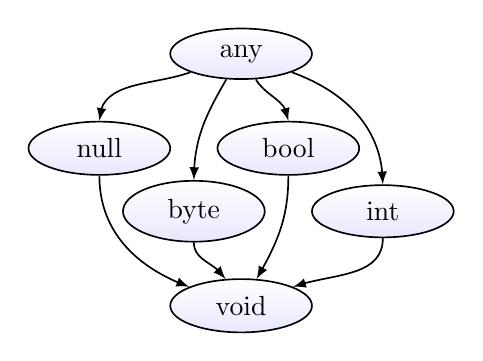
\begin{tikzpicture}[-latex, semithick , state/.style ={ellipse, top color = white, bottom color = #1!10, draw, black, text=black, minimum width = 1.8 cm, minimum height = 0.5 cm, align = left}]
	%\scriptsize
	
	\node[state={c1515F0},align=center] (A) at (3,4) {any};
	\node[state={c1515F0},align=center] (B) at (1.2,2.8) {null};
	\node[state={c1515F0},align=center] (C) at (2.4,2) {byte};
	\node[state={c1515F0},align=center] (D) at (3.6,2.8) {bool};
	\node[state={c1515F0},align=center] (E) at (4.8,2) {int};
	\node[state={c1515F0},align=center] (F) at (3,0.8) {void};
	\path (A) edge [in=90, out=-160] (B);
	\path (A) edge [in=90, out=-120] (C);
	\path (A) edge [in=90, out=-60] (D);
	\path (A) edge [in=90, out=-20] (E);
	\path (B) edge [in=160, out=-90] (F);
	\path (C) edge [in=120, out=-90] (F);
	\path (D) edge [in=60, out=-90] (F);
	\path (E) edge [in=20, out=-90] (F);
	\normalsize
	\end{tikzpicture}
	\caption{Lattice of primitive types}
\end{wrapfigure}

New types are constructed using :

\begin{itemize}
	\item \textbf{Primitive types} : (non-exhaustive list) \\
	\code {any} $=~\val$,\\
	\code {null} $=~\{null\}$,~~ \code {bool} $=~\{true, false\}$,\\ \code {byte} $=~\{0,1\}^8$,~~ \code {int} $=~\mathbb Z$,\\
	\code {void} $=~\emptyset$
	\item \textbf{Constructed types} : Records, Arrays, References, Functions or Methods.
	\item \textbf{Type operators} : Negation, intersection and union.
\end{itemize}



\paragraph{Constrained type}\pindent

The syntax \lstinline[language=Whiley,basicstyle=\normalsize\ttfamily]{define nat as (int x) where x >= 0}  enables to define types using previously declared ones and adding to them some constraints on the possible values. The use of a value that does not meet constraints will result in a compile time error.





\paragraph{Effective types} \pindent

To improve convenience, union of types that share the same structure (records, arrays, ...) exposes this common structure to. For example, the union of records that all have a field \code f is an effective record containing a field \code f of type the union of type for this field in the records.

%\paragraph{Functions or methods} \pindent
\label{EffTypes}

%A distinction is made between function that cannot have any side-effects and methods that can. 

\begin{wrapfigure}[8]{r}{0.45\textwidth}
	\vspace{-.5cm}
\begin{lstlisting}[language=Whiley]
function toBool(int|bool c) -> bool:
  if c is int:    // int|bool & int
    return c != 0 //   c : int
  else:           // int|bool & !int 
    return c      //   c : bool
\end{lstlisting}
\label{FlowTEC}
\end{wrapfigure}

\subsection{Flow-typing}
\label{FlowTE}
\indent

The Whiley language provides flow-typing that enable a variable to hold different types through the code. 
Type checking is introduced with the \whileyLine{is} operator. When used in a \whileyLine {if} statement, it refines the type of the checked variable on each branch, with enable to use them without cast. \\

The above code shows how variable's type is constructed on each branches of the \whileyLine {if} statement, using negation and intersection operators. the \whileyLine {return} line comments show the simplified type of \whileyLine{c}.

\subsection{The Compiler Collection}
\indent

Whiley sources are first converted to Whiley Intermediate Language (Wyil) by the front-end compiler (wyc). Wyil bytecodes are then given to back-end compilers. \\

Wyc handles lexing, parsing and type checking of Whiley sources. It also fully resolves names, giving each variable of a function a unique identifier. \autoref{wvcc} shows some of existing backends.

\begin{figure}[h]
	\center
	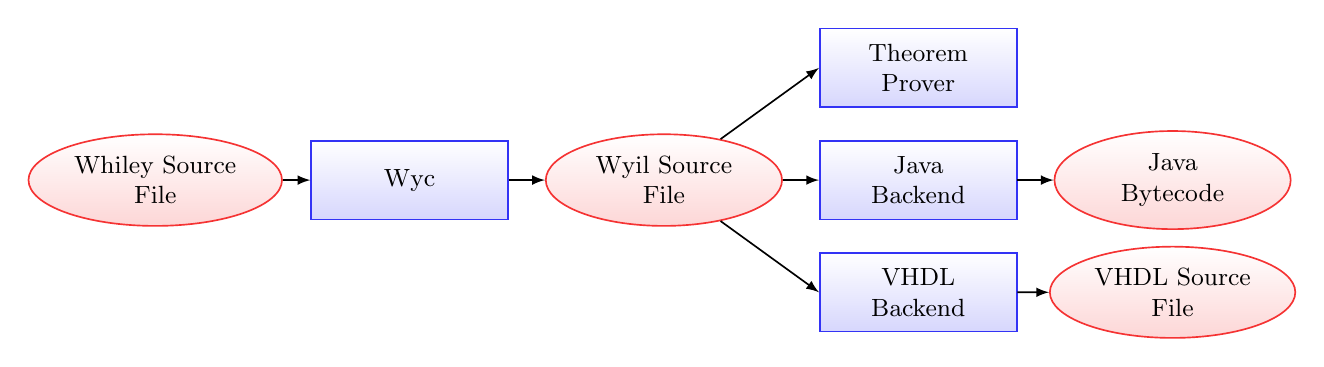
\begin{tikzpicture}[scale=.95,->, -latex, semithick , state/.style ={rectangle, top color = white, bottom color = processblue!20, draw, processblue, text=black, minimum width = 2.5 cm, minimum height = 1.0 cm, align = left}, stateB/.style ={ellipse, top color = white, bottom color = processred!20, draw, processred, text=black, minimum width = 3 cm, minimum height = 0.5 cm, align = left}]
	\small
	\node[stateB,align=center] (A) at (0,0) {Whiley Source \\ File};
	\node[state,align=center] (B) at (3.4,0) {Wyc};
	\node[stateB,align=center] (C) at (6.8,0) {Wyil Source \\ File};
	\node[state,align=center] (D) at (10.2,0) {Java \\ Backend};
	\node[stateB,align=center] (E) at (13.6,0) {Java\\ Bytecode};
	\node[state,align=center] (F) at (10.2,-1.5) {VHDL \\ Backend};
	\node[stateB,align=center] (G) at (13.6,-1.5) {VHDL Source \\ File};
	\node[state,align=center] (H) at (10.2,1.5) {Theorem \\ Prover};
	\draw (A) -- (B);
	\draw (B) -- (C);
	\draw (C) -- (D);
	\draw (D) -- (E);
	\draw (C) -- (F.west);
	\draw (F) -- (G);
	\draw (C) -- (H.west);

	\normalsize
	\end{tikzpicture}
	\caption{The Compiler Collection}
	\label{wvcc}
\end{figure}

This structure greatly simplifies the work of back-end compilers by gathering common part of the compilation process (lexing, parsing, typing) and giving back-end compilers only well formed and typed programs. 







\newpage
\section{The WhileyToVHDL Compiler}\indent

As part of this study, a new back-end compiler was developed : the WhileyToVHDL compiler that compiles Wyil bytecode to VHDL source files. It was constructed without any modifications of the langage but keeping in mind that extensions could be proposed.

\subsection{Overview}

\paragraph{Compilation process}\pindent

%\begin{wrapfigure}[20]{r}{0.35\textwidth}
%	\vspace{-1cm}
%	\center
%	\begin{tikzpicture}[-latex, semithick , state/.style ={rectangle, top color = white, bottom color = #1!10, draw, black, text=black, minimum width = 1.8 cm, minimum height = 0.5 cm, align = left}]
%	\small
%	
%	\node[state={c1515F0},align=center] (A) at (0,8) {Wyil Source \\ File};
%	\node[state={cF0F015},align=center] (B) at (0,6.5){Data-flow graph \\ building};
%	\node[state={cF0F015},align=center] (C) at (0,5) {Data-flow graph \\ optimizations};
%	\node[state={cF0F015},align=center] (D) at (0,3.5) {VHDL code \\ production};
%	\node[state={c1515F0},align=center] (E) at (0,2) {VHDL Source \\ File};
%	\path (A) edge  (B);
%	\path (B) edge  (C);
%	\path (C) edge  (D);
%	\path (D) edge  (E);
%	\normalsize
%	\end{tikzpicture}
%	\caption{Compilation pipeline}
%\end{wrapfigure}


Because of the source and targeted languages, the compilation process has several specific traits :

\begin{itemize}
	\item It is only a back-end compiler : no need to handle type checking nor verification, the input sources are supposed to be well formed and correct.
	\item The conversion of a sequential code to a hardware description (intrinsically parallel) requires the use of a specific transformation pipeline.
\end{itemize}

For each function, the compilation is achieved using the following steps :

\begin{figure}[h]
	\center
	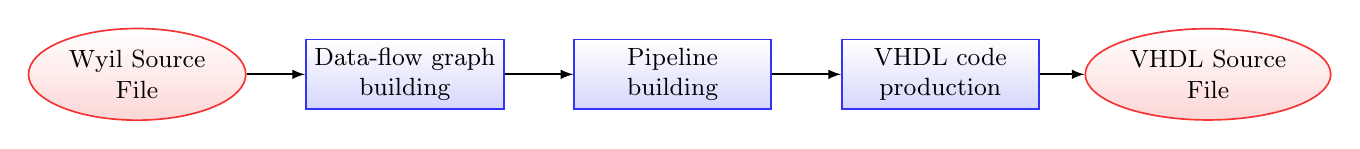
\begin{tikzpicture}[-latex, semithick , state/.style ={rectangle, top color = white, bottom color = processblue!20, draw, processblue, text=black, minimum width = 2.5 cm, minimum height = 0.5 cm, align = left}, stateB/.style ={ellipse, top color = white, bottom color = processred!20, draw, processred, text=black, minimum width = 1.8 cm, minimum height = 0.5 cm, align = left}]
	\small
	\node[stateB,align=center] (A) at (0,0) {Wyil Source \\ File};
	\node[state,align=center] (B) at (3.4,0) {Data-flow graph \\ building};
	\node[state,align=center] (C) at (6.8,0) {Pipeline \\ building};
	\node[state,align=center] (D) at (10.2,0) {VHDL code \\ production};
	\node[stateB,align=center] (E) at (13.6,0) {VHDL Source \\ File};
	\path (A) edge  (B);
	\path (B) edge  (C);
	\path (C) edge  (D);
	\path (D) edge  (E);
	\normalsize
	\end{tikzpicture}
	\caption{The compilation pipeline}
\end{figure}

\textbf{\textsl{Remark :}} Wyil files do not contain only function declarations. Nominal types can also be declared. They are pre-treated and stored for future use (See \hyperref[Types]{Types compilation}).

\paragraph{Compilation units} \pindent

The structure of Whiley files is preserved in the following way :
\begin{itemize}
	\item Each file is compiled to a unique VHDL file
	\item Each function is compiled to a unique VHDL entity
\end{itemize}

\paragraph{Restrictions on the language}\pindent

Only a small subset of the Whiley language is supported by the WhileyToVHDL compiler. The limitations arise from two major reasons :

\begin{itemize}
	\item \textbf{FPGAs' limitations} : Some features (floating point numbers) can't be efficiently introduced.
	\item \textbf{The amount of time necessary to add some concepts} : Arrays, partial recursion support, ...
\end{itemize}

\paragraph{Data-flow graph}\pindent

This graph describes how data are modified through a series of statements. Every path on this graph shows a possible transformation chain of an entry. This representation exposes the fine-grained parallelism that was hidden by the sequential description of the computation \cite{cardoso2003compilation, tripp2007trident, putnam2008chimps}. \\



To ensure a maximum use of this parallelism, the data-flow graph is built with VHDL values as atomic components. It is thus necessary to :

\begin{itemize}
	\item Convert the Whiley typed variables to VHDL ones, choosing a representation for each type.
	\item Build the data-flow graph from the functions body with the types constructed above.
\end{itemize}

\paragraph{VHDL generation}\pindent

Because VHDL is a data-flow language, the compilation of data-flow graphs to VHDL sources is mainly a straight-forward translation of vertexes to VHDL concurrent statements. Process statements are only used to convert register vertexes. Signals are created at strategic locations, to avoid duplication of expressions.



\subsection{Types compilation}\indent
\label{Types}

The choice of representation for Whiley variables relies on the conversion of their type to a construction using VHDL types.

\subsubsection{Purposes, difficulties and limitations}
\indent


Contrary to a classical CPU execution environment where variables are compiled to memory addresses or registers, VHDL signals represent a bunch of wires. This simple fact has several severe consequences :

\begin{itemize}
	\item \textbf{Types must be finite} : When a value of type $T$ is expected, a only finite number of bits (wires) will be allocated for it and they must be enough to store every possible value of this type. Whiley unbounded \code {int} are thus impossible to handle, and neither is \code {any} or recursive types.
	
	\item \textbf{Type operations must be resolved} : Storing a value of type $T_1|T_2$ can't be achieved with a pointer on a value of type $T_1$ or $T_2$ and a check of the effective type at runtime. Instead, the representation of both types has to be contained in the representation of the union type, as well as a way to distinguish the effective type of the value.
	
	\item \textbf{Type representations should optimized} : Because of the space limitation on targeted devices, the most compact representation as possible should be used. Storing the type \{int a\}$|$\{int b\} with two distinct values of type int is not desirable, as only one of them will be useful.
\end{itemize}

The compilation of (finite) arrays was not studied. A simple work around would lies in representing arrays with records with array's length fields of array's type. 

\paragraph{Type representation}~\\\indent

When feasible, a Whiley type will be converted to a set of VHDL types that handles every possible value of this type. To make the processing easier and the produced code clearer, the different components of a type representation are organized in a tree. It also enables to easily create signals with unique names.
The complete discussion about the choices of theses representation can be found \hyperref[Repr]{below}.


\begin{figure}[H]
	\centering
	\small
	\subfloat[\code {\{bool a, int b\}}]{
		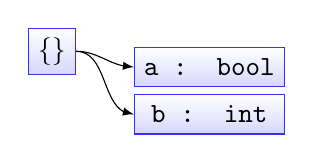
\begin{tikzpicture}
	
		
		\node[record] (A) at (3,-.4) {\code{\{\}}};
		\node[primitive] (AA) at (5,-.6) {\code {a : bool}};
		\node[primitive] (AB) at (5,-1.2) {\code {b : int}};
		
		\path (A.east) edge [out=-0, in=180] (AA.west);
		\path (A.east) edge [out=-0, in=180] (AB.west);
		
		\end{tikzpicture}
	}
	\hspace{.77cm}
	\subfloat[\code {bool|int}]{
		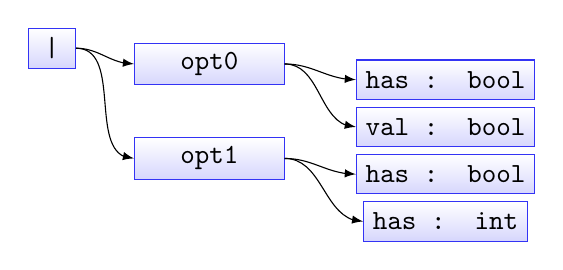
\begin{tikzpicture}
		
		\node[record] (A) at (3,-.4) {\code|};
		\node[primitive] (AA) at (5,-.6) {\code {opt0}};
		\node[primitive] (AAA) at (8,-.8) {\code {has : bool}};
		\node[primitive] (AAB) at (8,-1.4) {\code {val : bool}};
		\node[primitive] (AB) at (5,-1.8) {\code {opt1}};
		\node[primitive] (ABA) at (8,-2) {\code {has : bool}};
		\node[primitive] (ABB) at (8,-2.6) {\code {has : int}};
		
		\path (A.east) edge [out=-0, in=180] (AA.west);
		\path (AA.east) edge [out=-0, in=180] (AAA.west);
		\path (AA.east) edge [out=-0, in=180] (AAB.west);
		\path (A.east) edge [out=-0, in=180] (AB.west);
		\path (AB.east) edge [out=-0, in=180] (ABA.west);
		\path (AB.east) edge [out=-0, in=180] (ABB.west);
		
		\end{tikzpicture}
	}
	\normalsize
	\caption{Example of simple type representations}
\end{figure}

\textbf{\textsl{Remark :}} The case of Whiley's \code int type is resolved by fixing the size of integer (32 bits signed integers). To preserve Whiley semantic, an analysis of constraints of integer types could replace this solution, that would enable to adjust precisely the size of integers\cite{pearce2015integer}.




\paragraph{Type resolution}\pindent

Because some type constructions can't be easily represented with VHDL types (intersections, negations), types must be simplified when feasible to equivalent forms free of unsupported operations. \\

Such complex types arise when using \hyperref[FlowTE]{flow typing} : the types of variables on each branch are defined with intersections and negations. Because the front-end compiler simplify only basic cases, a deeper analysis was built to ensure the widest support of flow typing.


\subsubsection{Type analysis}
\indent

The simplification of type expressions is based on the elimination of redundant components in unions or intersections. Given a way to compare types, The simplification of type expressions can be achieved using the following facts :

\begin{itemize}
	\item If a component of a union is included in an other one, it is useless and removed from the union.
	\item If a component of an intersection contains an other one, it is useless and removed from the intersection.
	\item If two components of an intersection are disjointed, the resulting type is \whileyLine{void}.
	\item Union or intersection with only one option are converted to this unique component.
\end{itemize}

A canonical form is used to reveal possible simplifications. The analyse of above \hyperref[FlowTEC]{flow typing example} variable \whileyLine {c} in the \whileyLine {else} branch would work the following way :

\begin{figure}[h]
	\center
	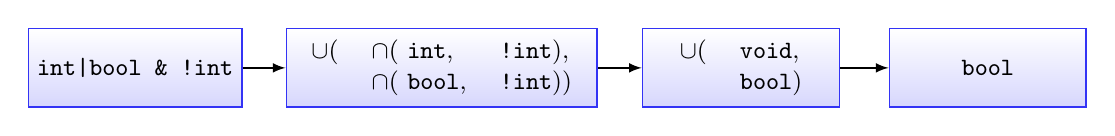
\begin{tikzpicture}[scale=.95,->, -latex, semithick , state/.style ={rectangle, top color = white, bottom color = processblue!20, draw, processblue, text=black, minimum width = 2.5 cm, minimum height = 1.0 cm, align = left},]
	\small
	\node[state,align=center] (A) at (0.3,0) {\code {int|bool \& !int}};
	\node[state,align=center] (B) at (4.4,0) {\begin{tabular}{rll}
		$\cup($ & $\cap($ \code{int}, & \code{!int}$),$ \\
		& $\cap($ \code{bool}, & \code{!int}$))$ 
	\end{tabular}};
	\node[state,align=center] (C) at (8.4,0) {\begin{tabular}{rl}
		$\cup($ & \code{void}$,$ \\
		& \code{bool}$)$ 
	\end{tabular}};
	\node[state,align=center] (D) at (11.7,0) {\code {bool}};
	\draw (A) -- (B);
	\draw (B) -- (C);
	\draw (C) -- (D);
	
	\normalsize
	\end{tikzpicture}
\end{figure}


In the following study,
\begin{itemize}
	\item $\val$ is the set of acceptable Whiley typed values (closed by Cartesian product)
	\item $\lea = $\{any, bool, byte, int, null, void\} is the set of primitive types
	\item Records are represented with Cartesian products: $\{T1~a,~T2~b\}~\equiv~T1 \times T2$, regardless field's names that are not relevant here.
\end{itemize}

\paragraph{The canonical form}~\\\indent

We denote with \textit{simple types} ($\mathcal S$) the set of primitive types and record types whose components are all simple types. Types are said \textit{in canonical form} if they are defined as :
\[
\bigcup_i \bigcap_j T_{i,j} , ~~ T_{i,j} \in \mathcal S \mbox{ or } T_{i,k} ~=~ \val \setminus S, ~ S \in \mathcal S
\]


Type expressions are transformed using the classical set equations :
\[
\begin{array}{rcl}
	\overline{\bigcup _k T_k} & = & \bigcap _k \overline{T_k} \\
	\overline{\bigcap _k T_k} & = & \bigcup _k \overline{T_k} \\
	\bigcap _{i \in  [ \! [ 1,n ] \! ] } \bigcup _{j \in J_i} T_{i,j} & = & \bigcup _{I \in J_1\times\ldots\times J_n} \bigcap _i T_{i, I_i}
\end{array}
\]

The case of records (Cartesian products) needs more care :
\[
T_1 \times (\overline{T_2}) ~ = ~ \left(T_1 \times \val \right) \cap \left( \overline{T_1 \times T_2} \right)
\]


\begin{figure}[h]
	\centering
	\begin{tabular}{|c|c|c|}
	\hline
	int & int$|$bool & \{int$|$bool~a,~!byte~b\} \\
	\hline
	$\cup(\cap($int$))$ & $\cup(\cap($int$),~\cap($bool$))$ & 
	\begin{tabular}{lll}
		$\cup($ & $\cap($\{int a, any b\}, & !\{int a, byte b\}$),$ \\
		& $\cap($\{bool a, any b\}, & !\{bool a, byte b\}$))$ 
	\end{tabular} \\
	\hline
	\end{tabular}
	\caption{Some canonical form examples}
\end{figure}

Because types \code{any} (\textit{resp.} \code{void}) is the neutral element for the intersection (\textit{resp.} union), the canonical form is not unique.


\begin{wrapfigure}[14]{r}{0.45\textwidth}
\vspace{-20pt}
\center
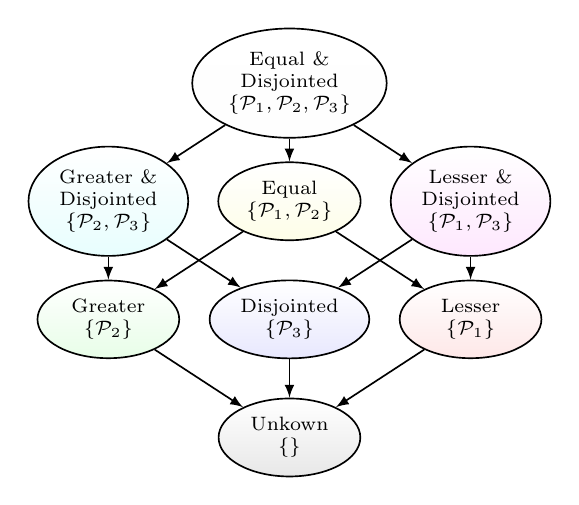
\begin{tikzpicture}[-latex, semithick , state/.style ={ellipse, top color = white, bottom color = #1!10, draw, black, text=black, minimum width = 1.8 cm, minimum height = 0.5 cm, align = left}]
\scriptsize
		
\node[state={c15F0F0},align=center] (X) at (1.7,4) {Greater \& \\ Disjointed\\$\{\mathcal P_2, \mathcal P_3\}$};
\node[state={cF0F0F0},align=center] (Y) at (4,5.5) {Equal \& \\ Disjointed\\$\{\mathcal P_1, \mathcal P_2, \mathcal P_3\}$};
\node[state={cF015F0},align=center] (Z) at (6.3,4) {Lesser \& \\ Disjointed\\$\{\mathcal P_1, \mathcal P_3\}$};

\node[state={c1515F0},align=center] (A) at (4,2.5) {Disjointed\\$\{\mathcal P_3\}$};
\node[state={cF0F015},align=center] (B) at (4,4) {Equal\\$\{\mathcal P_1, \mathcal P_2\}$};
\node[state={c15F015},align=center] (C) at (1.7,2.5) {Greater\\$\{\mathcal P_2\}$};
\node[state={cF01515},align=center] (D) at (6.3,2.5) {Lesser\\$\{\mathcal P_1\}$};
\node[state={c151515},align=center] (E) at (4,1) {Unkown\\$\{\}$};
\path (X) edge  (C);
\path (Y) edge  (B);
\path (Y) edge  (X);
\path (Y) edge  (Z);
\path (Z) edge  (D);
\path (X) edge  (A);
\path (Z) edge  (A);
\path (A) edge  (E);
\path (B) edge  (C);
\path (B) edge  (D);
\path (C) edge  (E);
\path (D) edge  (E);
\normalsize
\end{tikzpicture}
\caption{Lattice of comparison results}
\label{Latt}
\end{wrapfigure}



\paragraph{Type comparison}~\\\indent


The implemented comparison between $T_1$ and $T_2$ is achieved trying to check the following properties :
\begin{itemize}
\item $\mathcal P_1$ : $T_1 \subset T_2$
\item $\mathcal P_2$ : $T_2 \subset T_1$
\item $\mathcal P_3$ : $T_1 \cap T_2 = \emptyset$
\end{itemize}

Theses properties can independently be effective or not. (If the three properties are true, both types are necessarily empty)\\


A result of comparison is the set of properties that are known to be true. \autoref{Latt} gives a name to the different results and shows their implication. Testing a subtype relation is done by checking if $\mathcal P_1$ or $\mathcal P_2$ is known to be true in the result of the comparison.\\



The comparison of two types is computed in the following way :
\begin{itemize}
	\item If both of the types are primitive types, the result is well defined (Equal if they are the same, included if one of them is \whileyLine{any} and disjointed in the remaining cases except if one of them is \whileyLine {void} where a more precise result is available). 
	\item If one of them is a constructed type, its components are compared to the other and the result is build using some merging rules on components comparison's results.
\end{itemize}


%
%\begin{figure}
%	\begin{tabular}{}
%		content...
%	\end{tabular}}
%	\caption {The union rule}
%\end{figure}










To keep more information during comparison, a fourth dimension could be added, corresponding to the property $\mathcal P_4$ : $T_1 \cup T_2 = \val$.\\

%
%In the following description, $T_1,~T_2,~T_3,~T_4$ denote types and $o,~o_1,~o_2$ comparison results.\\
%
%This comparison result between two types $T_1$ and $T_2$ will be denoted $T_1/T_2$. The relation $o_1 \trianglelefteq o_2$ on $\ord$ intuitively means that the order $o_1$ is \textit{more} precise than $o_2$. \\
%
%The comparison is built using a structural induction : the comparison results are known for primitive types, and built type are compared using the following functions :
%
%\begin{itemize}
%\item \textbf{Opposite} ($Opp$) : 
%\[
%\dfrac{T_1}{T_2} \trianglelefteq o \implies \dfrac{T_2}{T_1} \trianglelefteq Opp(o)
%\]
%\item \textbf{Negation} ($Neg$) :
%\[
%\dfrac{T_1}{T_2} \trianglelefteq o \implies \dfrac{!T_1}{!T_2} \trianglelefteq Neg(o)
%\]
%\item \textbf{Semi-negation} ($Sng$) :
%\[
%\dfrac{T_1}{T_2} \trianglelefteq o \implies \dfrac{!T_1}{T_2} \trianglelefteq Sng(o)
%\]
%\item \textbf{Conjunction} ($Con$) :
%\[
%\dfrac{T_1}{T_2} \trianglelefteq o_1, ~ \dfrac{T_3}{T_4} \trianglelefteq o_2,~
%\left\lbrace
%\begin{array}{lll}
%T_1\cap T_3 & = & \varnothing\\
%T_2\cap T_4 & = & \varnothing
%\end{array}\right.  \implies \dfrac{T_1 | T_2}{T_3 | T_4} \trianglelefteq Con(o_1, o_2)
%\]
%\item \textbf{Union} ($Uni$) :
%\[
%\dfrac{T_1}{T_3} \trianglelefteq o_1, ~ \dfrac{T_2}{T_3} \trianglelefteq o_2 \implies \dfrac{T_1|T_2}{T_3} \trianglelefteq Uni(o_1, o_2)
%\]
%\item \textbf{Intersection} ($Int$) :
%\[
%\dfrac{T_1}{T_3} \trianglelefteq o_1, ~ \dfrac{T_2}{T_3} \trianglelefteq o_2 \implies \dfrac{T_1\&T_2}{T_3} \trianglelefteq Int(o_1, o_2)
%\]
%\item \textbf{Precision} ($Pre$) :
%\[
%\dfrac{T_1}{T_2} \trianglelefteq o_1, ~ \dfrac{T_1}{T_2} \trianglelefteq o_2 \implies \dfrac{T_1\&T_2}{T_3} \trianglelefteq Pre(o_1, o_2), \left\lbrace
%\begin{array}{lll}
%Pre(o_1, o_2) & \trianglelefteq & o_1\\
%Pre(o_1, o_2) & \trianglelefteq & o_2
%\end{array}\right.
%\]
%\end{itemize}
%
%The conjunction rule is used to compare records were each field are independent of the others.
%
%Some of these relations seems redundant, but it appears that this has to be carefully studied. In the case of the 3 dimensions comparison lattice, the following results can be observed :
%
%\[
%\forall o, ~ \left\lbrace \begin{array}{lll}
%Neg(o) & \trianglelefteq & Sng\left(Opp\left(Sng\left(Opp\left(o\right)\right)\right)\right) \\
%Neg(o) & \trianglelefteq & Opp\left(Sng\left(Opp\left(Sng\left(o\right)\right)\right)\right) 
%\end{array}\right.
%\]
%\[
%\left\lbrace \begin{array}{llllll}
%Neg(Greater) & = & Lesser, & Sng\left(Opp\left(Sng\left(Opp\left(Greater\right)\right)\right)\right) & = & Unknown \\
%Neg(Lesser) & = & Greater, &Opp\left(Sng\left(Opp\left(Sng\left(Lesser\right)\right)\right)\right) & = & Unknown \\
%\end{array}\right.
%\]
%
%
%The lesser accuracy of the alternative expressions is due to the fact that $Sng(Lesser) = Unknown$.
%The complete precision can be recovered using :
%\[
%\forall o, ~ Neg(o) ~ = ~ Pre\left( Sng\left(Opp\left(Sng\left(Opp\left(o\right)\right)\right)\right), Opp\left(Sng\left(Opp\left(Sng\left(o\right)\right)\right)\right) \right)
%\]
%
%
%To improve precision, the default comparison of $T_1$ against $T_2$ is computed with
%\[
%\Dfrac{T_1}{T_2} ~ = ~ Pre\left(\dfrac{T_1}{T_2}, Opp\left(\dfrac{T_2}{T_1}\right)\right)
%\]


\textbf{\textit{Remark}} : An other algorithm was proposed by D. J. Pearce \cite{SubTyping} to build the subtype operator, based on only computing the property $T_1 \cap T_2 ~=~ \emptyset$ ($\mathcal P_3$). A similar canonical form is used to ensure this operator can be constructed. Other comparison results can be then implemented using it :
\[
	T_1 \subset T_2 ~\Leftrightarrow~ T_1 \cap (\val \setminus T_2) = \emptyset
\]



%
%The comparison is asymmetrical : 
%
%\code {int|bool / (!int)\&(!bool)}
%
%\code {int|bool / (!int)\&(!bool)}
%\begin{figure}[h]
%\begin{tabular}{ccc}
%\begin{tikzpicture}[-latex, semithick , state/.style ={rectangle, top color = white, bottom color = processred!20, draw, processblue, text=blue, minimum height = 0.5 cm, align = left}, stateB/.style ={circle, top color = white, bottom color = processred!5, draw, processblue, text=blue, minimum height = 0.5 cm, align = left}]
%\small
%		
%\node[state,align=center] (A) at (2,7) {$\dfrac{(!int)\&(!bool)}{int|bool}$};
%\node[state,align=center] (AA) at (0,5.5) {$\dfrac{!int}{int|bool}$};
%\node[state,align=center] (AB) at (4,5.5) {$\dfrac{!bool}{int|bool}$};
%\node[state,align=center] (AAA) at (-1,4) {$\dfrac{!int}{int}$};
%\node[state,align=center] (AAB) at (1,4) {$\dfrac{!int}{bool}$};
%\node[state,align=center] (ABA) at (3,4) {$\dfrac{!bool}{int}$};
%\node[state,align=center] (ABB) at (5,4) {$\dfrac{!bool}{bool}$};
%
%\node at (0,2.5) {$|$};
%\node at (4,2.5) {$|$};
%\node at (2,1.5) {$\&$};
%
%\node[stateB,align=center] (B) at (2,0.5) {$?$};
%\node[stateB,align=center] (BA) at (0,1.5) {$?$};
%\node[stateB,align=center] (BB) at (4,1.5) {$?$};
%\node[stateB,align=center] (BAA) at (-1,2.5) {$\bowtie$};
%\node[stateB,align=center] (BAB) at (1,2.5) {$?$};
%\node[stateB,align=center] (BBA) at (3,2.5) {$?$};
%\node[stateB,align=center] (BBB) at (5,2.5) {$\bowtie$};
%
%\path (A) edge  (AA);
%\path (A) edge  (AB);
%\path (AA) edge  (AAA);
%\path (AA) edge  (AAB);
%\path (AB) edge  (ABA);
%\path (AB) edge  (ABB);
%
%\path (AAA) edge  (BAA);
%\path (AAB) edge  (BAB);
%\path (ABA) edge  (BBA);
%\path (ABB) edge  (BBB);
%
%\path (BA) edge  (B);
%\path (BB) edge  (B);
%\path (BAA) edge  (BA);
%\path (BAB) edge  (BA);
%\path (BBA) edge  (BB);
%\path (BBB) edge  (BB);
%
%\normalsize
%\end{tikzpicture}
%&~~&
%\begin{tikzpicture}[-latex, semithick , state/.style ={rectangle, top color = white, bottom color = processred!20, draw, processblue, text=blue, minimum height = 0.5 cm, align = left}, stateB/.style ={circle, top color = white, bottom color = processred!20, draw, processblue, text=black, minimum height = 0.5 cm, align = left}]
%\small
%		
%\node[state,align=center] (A) at (2,7) {$\dfrac{int|bool}{(!int)\&(!bool)}$};
%\node[state,align=center] (AA) at (0,5.5) {$\dfrac{int}{(!int)\&(!bool)}$};
%\node[state,align=center] (AB) at (4,5.5) {$\dfrac{bool}{(!int)\&(!bool)}$};
%\node[state,align=center] (AAA) at (-1,4) {$\dfrac{int}{!int}$};
%\node[state,align=center] (AAB) at (1,4) {$\dfrac{int}{!bool}$};
%\node[state,align=center] (ABA) at (3,4) {$\dfrac{bool}{!int}$};
%\node[state,align=center] (ABB) at (5,4) {$\dfrac{bool}{!bool}$};
%
%\node at (0,2.5) {$\&$};
%\node at (4,2.5) {$\&$};
%\node at (2,1.5) {$|$};
%
%\node[stateB,align=center] (B) at (2,0.5) {$\bowtie$};
%\node[stateB,align=center] (BA) at (0,1.5) {$\bowtie$};
%\node[stateB,align=center] (BB) at (4,1.5) {$\bowtie$};
%\node[stateB,align=center] (BAA) at (-1,2.5) {$\bowtie$};
%\node[stateB,align=center] (BAB) at (1,2.5) {$?$};
%\node[stateB,align=center] (BBA) at (3,2.5) {$?$};
%\node[stateB,align=center] (BBB) at (5,2.5) {$\bowtie$};
%
%\path (A) edge  (AA);
%\path (A) edge  (AB);
%\path (AA) edge  (AAA);
%\path (AA) edge  (AAB);
%\path (AB) edge  (ABA);
%\path (AB) edge  (ABB);
%
%\path (AAA) edge  (BAA);
%\path (AAB) edge  (BAB);
%\path (ABA) edge  (BBA);
%\path (ABB) edge  (BBB);
%
%\path (BA) edge  (B);
%\path (BB) edge  (B);
%\path (BAA) edge  (BA);
%\path (BAB) edge  (BA);
%\path (BBA) edge  (BB);
%\path (BBB) edge  (BB);
%
%\normalsize
%\end{tikzpicture}
%\end{tabular}
%\end{figure}



\subsubsection{Type representation} \indent
\label{Repr}

Once the types have been simplified, if they do not contain any intersection, negation or infinite types, they are converted to a tree which leaves are primitive types.

\paragraph{Primitive types}~\\\indent

The leaves of this tree are VHDL types that can represent a Whiley type in an obvious manner. They are drawn in red on the following diagrams.

\begin{itemize}
	\item \code{int} are represented with \code{signed(31 downto 0)}
	\item \code{bool} are represented with \code{boolean}
	\item \code{byte} are represented with \code{std\_logic\_vector(7 downto 0)}
\end{itemize}

\paragraph{Complex types}~\\\indent


To build the other types, several kind of inner nodes are provided. Some of them do not correspond to any Whiley construction, but enable an easy compilation of type related operations :

\newlength{\pict}
\setlength{\pict}{.22\textwidth}

\begin{itemize}
	\item[] 
	\begin{minipage}[b]{.95\textwidth}
		%\vspace{-.01cm}
		\begin{wrapfigure}{r}{\pict}
			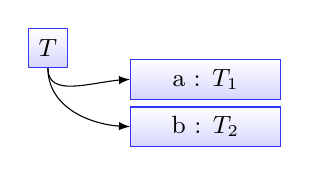
\begin{tikzpicture}
			\small
			
			\node[root] (A) at (0,0) {$T$};
			
			\node[primitive] (B) at (2,-.4) {a : $T_1$};
			\node[primitive] (C) at (2,-1) {b : $T_2$};
			\path (A.south) edge [out=-90, in=180] (B.west);
			\path (A.south) edge [out=-90, in=180] (C.west);
			\normalsize
			\end{tikzpicture}
		\end{wrapfigure}
		~%\vspace{.01cm}
		\item \textbf{Record nodes} : Each field is stored in a sub tree labelled with its name.
		\begin{flushright}
			Type $T$ : {\{$T_1$ a, $T_2$ b\}}
		\end{flushright}
	\end{minipage} 
	
	\item[] 
	\begin{minipage}[b]{.95\textwidth}
		%\vspace{-.01cm}
		\begin{wrapfigure}{r}{\pict}
			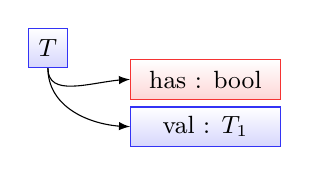
\begin{tikzpicture}
			\small
			
			\node[root] (A) at (0,0) {$T$};
			
			\node[leaf] (B) at (2,-.4) {has : bool};
			\node[primitive] (C) at (2,-1) {val : $T_1$};
			\path (A.south) edge [out=-90, in=180] (B.west);
			\path (A.south) edge [out=-90, in=180] (C.west);
			\normalsize
			\end{tikzpicture}
		\end{wrapfigure}
		~%\vspace{.01cm}
		\item \textbf{Option nodes} : Add a boolean flag to a type, intended to indicate if the value is meaningful or not. Theses nodes are used by other inner nodes.
		\begin{flushright}
			Type $T$ : $T_1?$
		\end{flushright}
	\end{minipage} 
	
	\item[] 
	\begin{minipage}[b]{.95\textwidth}
		%\vspace{-.01cm}
		\begin{wrapfigure}{r}{\pict}
			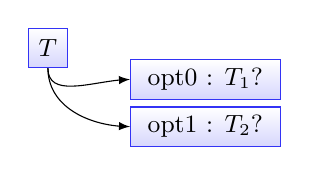
\begin{tikzpicture}
			\small
			
			\node[root] (A) at (0,0) {$T$};

			\node[primitive] (B) at (2,-.4) {opt0 : $T_1?$};
			\node[primitive] (C) at (2,-1) {opt1 : $T_2?$};
			\path (A.south) edge [out=-90, in=180] (B.west);
			\path (A.south) edge [out=-90, in=180] (C.west);
			\normalsize
			\end{tikzpicture}
		\end{wrapfigure}
		~%\vspace{.01cm} 
		\item \textbf{Primitive union nodes} : If every option's components is a primitive type, a tree with one option sub tree per component is built.
		\begin{flushright}
			Type $T$ : $T_1|_pT_2$
		\end{flushright}
	\end{minipage} 
	
	\item[] 
	\begin{minipage}[b]{.95\textwidth}
		%\vspace{-.01cm}
		\begin{wrapfigure}{r}{\pict}
			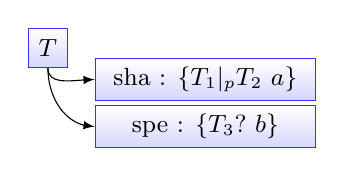
\begin{tikzpicture}
			\small
			
			\node[root] (A) at (0,0) {$T$};
			
			\node[primitive,minimum width = 2.8cm] (B) at (2,-.4) {sha : $\{T_1|_pT_2~a\}$};
			\node[primitive,minimum width = 2.8cm] (C) at (2,-1) {spe : $\{T_3?~b\}$};
			\path (A.south) edge [out=-90, in=180] (B.west);
			\path (A.south) edge [out=-90, in=180] (C.west);
			\normalsize
			\end{tikzpicture}
		\end{wrapfigure}
		~%\vspace{.01cm}
		\item \textbf{Record union nodes} : Gather identically named fields and store specific ones with an option sub tree.
		\begin{flushright}
			Type $T$ : $\{T_1~a\}|_r\{T_2 ~a,~T_3~b\}$
		\end{flushright}
	\end{minipage} 
	
	\item[] 
	\begin{minipage}[b]{.95\textwidth}
		%\vspace{-.01cm}
		\begin{wrapfigure}{r}{\pict}
			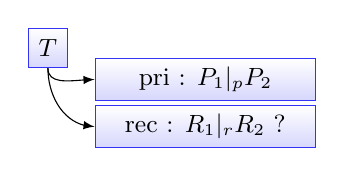
\begin{tikzpicture}
			\small
			
			\node[root] (A) at (0,0) {$T$};
			
			\node[primitive,minimum width = 2.8cm] (B) at (2,-.4) {pri : $P_1|_pP_2$};
			\node[primitive,minimum width = 2.8cm] (C) at (2,-1) {rec : $R_1|_rR_2 ~?$};
			\path (A.south) edge [out=-90, in=180] (B.west);
			\path (A.south) edge [out=-90, in=180] (C.west);
			\normalsize
			\end{tikzpicture}
		\end{wrapfigure}
		~%\vspace{.01cm}
		\item \textbf{General union nodes} : Store a general union, separating records options from primitive ones.
		\begin{flushright}
			Type $T$ : $P_1|P_2|R_1|R_2$
		\end{flushright}
	\end{minipage} 
\end{itemize}


Some primitive types are not straightforwardly convertible to VHDL values :


\begin{itemize}
	\item The type \code {null} is converted to an empty record : the only value of type \code Null is null, so no bits are needed to store it. This type is useful when part of a union (\code {int|null}), and the boolean of the option is the holding the information.
	\item The type \code {void} is not convertible because it contains no values.
	\item The distinction between simple unions and records unions was introduced to easily handle Whiley's \hyperref[EffTypes]{effective types}.
\end{itemize}


\begin{figure}[h]
	\centering
	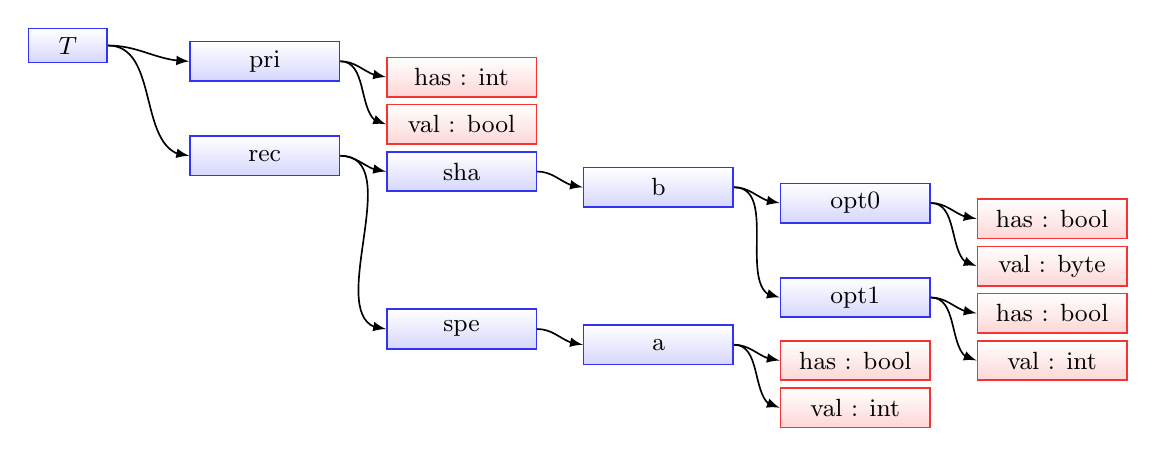
\begin{tikzpicture}[-latex, semithick , state/.style ={rectangle, top color = white, bottom color = processblue!20, draw, processblue, text=blue, minimum width = 4.5 cm, minimum height = 0.5 cm}]
	\small
	
	\node[rectangle ,top color =white , bottom color = processblue!20 ,
	draw,processblue , text=black , minimum width =1 cm] (A) at (-.5,.6) {$T$};
	
	\node[primitive] (B) at (2,.4) {pri};
	\node[leaf] (BA) at (4.5,.2) {has : int};
	\node[leaf] (BB) at (4.5,-.4) {val : bool};
	\node[primitive] (C) at (2,-.8) {rec};
	\node[primitive] (CA) at (4.5,-1) {sha};
	\node[primitive] (CAA) at (7,-1.2) {b};
	\node[primitive] (CAAA) at (9.5,-1.4) {opt0};
	\node[leaf] (CAAAA) at (12,-1.6) {has : bool};
	\node[leaf] (CAAAB) at (12,-2.2) {val : byte};
	\node[primitive] (CAAB) at (9.5,-2.6) {opt1};
	\node[leaf] (CAABA) at (12,-2.8) {has : bool};
	\node[leaf] (CAABB) at (12,-3.4) {val : int};
	\node[primitive] (CB) at (4.5,-3) {spe};
	\node[primitive] (CBA) at (7,-3.2) {a};
	\node[leaf] (CBAA) at (9.5,-3.4) {has : bool};
	\node[leaf] (CBAB) at (9.5,-4) {val : int};
	
	\path (A.east) edge [out=-0, in=180] (B.west);
	\path (B.east) edge [out=-0, in=180] (BA.west);
	\path (B.east) edge [out=-0, in=180] (BB.west);
	\path (A.east) edge [out=-0, in=180] (C.west);
	\path (C.east) edge [out=-0, in=180] (CA.west);
	\path (CA.east) edge [out=-0, in=180] (CAA.west);
	\path (CAA.east) edge [out=-0, in=180] (CAAA.west);
	\path (CAAA.east) edge [out=-0, in=180] (CAAAA.west);
	\path (CAAA.east) edge [out=-0, in=180] (CAAAB.west);
	\path (CAA.east) edge [out=-0, in=180] (CAAB.west);
	\path (CAAB.east) edge [out=-0, in=180] (CAABA.west);
	\path (CAAB.east) edge [out=-0, in=180] (CAABB.west);
	\path (C.east) edge [out=-0, in=180] (CB.west);
	\path (CB.east) edge [out=-0, in=180] (CBA.west);
	\path (CBA.east) edge [out=-0, in=180] (CBAA.west);
	\path (CBA.east) edge [out=-0, in=180] (CBAB.west);
	\normalsize
	\end{tikzpicture}
	\caption{Representation of type $T$ : \{int a, byte b\}$|$\{int b\}$|$int }
\end{figure}


\textbf{\textsl{Remark :}} Recursive types such as trees are not convertible as they may describe values of unknown and unbound size.





\subsection{Building the data-flow graph}
\indent

The building of the data-flow graph transforms the function body to a graph exposing the paths data can follow during the execution. 


\subsubsection{Vertexes}
\indent

Because Whiley types are converted to a tree of VHLD types, each Whiley variable is associated with a tree with vertexes as leaves that represent its current state. \\

This graph is made of two types of vertexes : 
\begin{itemize}
	\item \textbf{Symbolic vertexes} : represent constants or inputs/outputs (of the function or the called functions). They have at most one source.
	\item \textbf{Operation vertexes} : represent operations, with their operands as sources. Complex operations are compiled to equivalent set of basic operations (see the \hyperref[FlowT]{\code {is} operator}).
\end{itemize}



When meaningful, vertexes are typed with a VHDL type, Only these kind of vertexes can then be compiled toward VHDL statements.



\subsubsection{Compiling the function body} \indent

To compile a function body, a map of Whiley variables to the current tree of vertexes representing them is stored and initialized with input nodes for each argument. Body's statements are then successively processed to construct the graph. Some worth-mentioning statements are discuss below.

\paragraph{Variable assignments}\pindent


The compilation of variable assignments modifies the tree of vertexes that represents the assigned variable. It requires three steps and \autoref{Assign} illustrates the different nodes that are created.


\newbox\assign
\begin{lrbox}{\assign}
	\begin{minipage}[t]{.35\textwidth}
\begin{lstlisting}[language=Whiley]
type T is {bool|int a, byte b}
		
function answer(T t) -> T:
    t.a = 42
    return t
\end{lstlisting}
	\end{minipage}
\end{lrbox}

\begin{figure}[h]
	\centering
	\subfloat[Assignment statement]{\adjustbox{valign=b}{\usebox\assign}}
	\qquad \subfloat[Tree respresenting t after assignment]{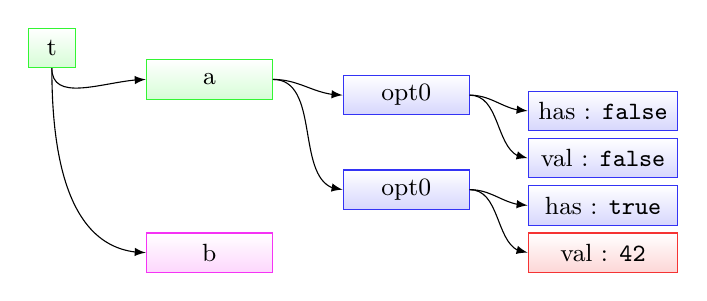
\begin{tikzpicture}
		\small
		
		\node[general={processgreen}{.6}] (A) at (0,0) {t};
		
		\node[general={processgreen}{1.6}] (B) at (2,-.4) {a};
		\node[general={processblue}{1.6}] (BA) at (4.5,-.6) {opt0};
		\node[general={processblue}{1.9}] (BAA) at (7,-.8) {has : \code{false}};
		\node[general={processblue}{1.9}] (BAB) at (7,-1.4) {val : \code{false}};
		\node[general={processblue}{1.6}] (BB) at (4.5,-1.8) {opt0};
		\node[general={processblue}{1.9}] (BBA) at (7,-2) {has : \code{true}};
		\node[general={processred}{1.9}] (BBB) at (7,-2.6) {val : \code{42}};
		\node[general={processpurple}{1.6}] (C) at (2,-2.6) {b};
		\path (A.south) edge [out=-90, in=180] (B.west);
		\path (A.south) edge [out=-90, in=180] (C.west);
		\path (B.east) edge [out=-0, in=180] (BA.west);
		\path (BA.east) edge [out=-0, in=180] (BAA.west);
		\path (BA.east) edge [out=-0, in=180] (BAB.west);
		\path (B.east) edge [out=-0, in=180] (BB.west);
		\path (BB.east) edge [out=-0, in=180] (BBA.west);
		\path (BB.east) edge [out=-0, in=180] (BBB.west);
		\normalsize
		\end{tikzpicture}}
	\caption {Example of assignment}
	\label{Assign}
\end{figure}

\begin{enumerate}
	\item \textbf{Building of the right hand side} : A tree representing the \fcolorbox{processred}{processred!10}{new value} is built by compiling the expression. (\whileyLine{42} is represented with a simple integer vertex). 
	\item \textbf{Adjusting types} : Some \fcolorbox{processblue}{processblue!10}{additional signals} can be created to make the type of the expression fit the assign variable's one (\whileyLine{int} value must be adapted to be of \whileyLine{t.a}'s \whileyLine{int|bool} type).
	\item \textbf{Modifying trees} : Building the global tree of the modified variable, keeping some \fcolorbox{processpurple}{processpurple!10}{old sub-trees} and building \fcolorbox{processgreen}{processgreen!10}{new inner nodes} (\whileyLine{t.b} was not modified and should be kept).
\end{enumerate}




\paragraph{Function invocations}\pindent

Function calls are compiled to a special untyped vertex that contains necessary details about the function. It has as many sources as the function's arguments and its only targets are special symbolic vertexes that represent the return values of the function. During the production of VHDL code, the vertex is converted to a \hyperref[Concurr]{component instantiation}.


\paragraph{\code{If} statements and returns}\pindent

\newbox\ifm
\begin{lrbox}{\ifm}
	\begin{minipage}[t]{.322\textwidth}
\begin{lstlisting}[language=Whiley]
function s(int a) -> int:
    if a%2 == 0:
        a = a/2
    else:
        a = 3*a+1
    return a
\end{lstlisting}
	\end{minipage}
\end{lrbox}
\newbox\ifn
\begin{lrbox}{\ifn}
\begin{minipage}[t]{.322\textwidth}
\begin{lstlisting}[language=Whiley,showlines=true]
function s(int a) -> int:
    if a%2 == 0:
        return a/2
    return 3*a+1
    
    
\end{lstlisting}
\end{minipage}
\end{lrbox}

\begin{figure}[h]
	\centering
	\begin{minipage}{.7\textwidth}
\quad Contrary to a usual compilation strategy that use conditional jump on relevant part of the program, both true and false branch, as well as the condition are compiled separately, using pre-statement variable's representations. Modified variables are then gathered using a multiplexer. \\

\quad Extra care has to be taken with the management of returns when several statements are used in different blocks: because only one bunch of output signals must be constructed, they are treated as if returns were stored in a variable that is returned at the end.

	
	~\subfloat[Multiples return]{\adjustbox{valign=b}{\usebox\ifn}}	
	\qquad	\subfloat[Unique return]{\adjustbox{valign=b}{\usebox\ifm}}
	\end{minipage}~~
	\begin{minipage}{.28\textwidth}
	\subfloat[Resulting data-flow graph]{\adjustbox{valign=b}{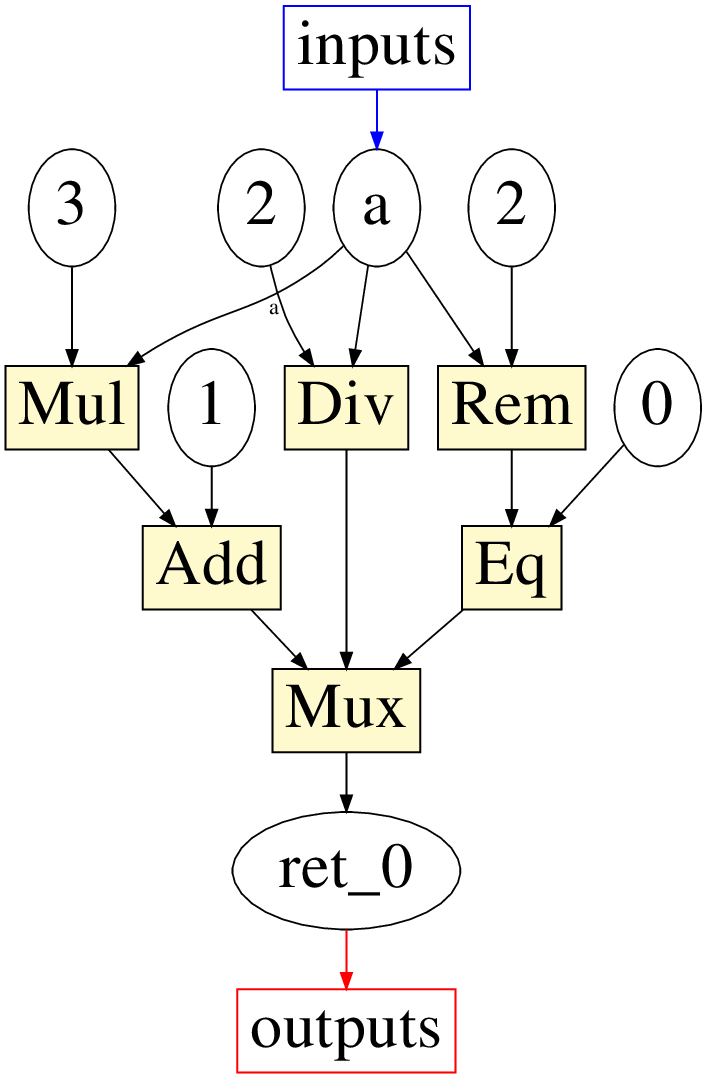
\includegraphics[scale=.23]{if.png}}}
	\end{minipage}
	\caption{If statement and multiple returns}
\end{figure}





\subsubsection{Flow typing}
\label{FlowT}\indent

Flow typing provides a very convenient way to deal with constructed types and its support relies mainly on the operator \code {is} and alias declarations.


\paragraph{Operator \code is}~\\\indent

Runtime type checking is mainly useful when dealing with union typed values. It is compiled using the additional flags that were added in option nodes : the expression \whileyLine {x is int} where \whileyLine {x} has type \whileyLine {int|bool} is converted to a simple reading of \whileyLine{int} option's \code {has} flag.

\paragraph{Aliases}~\\\indent

In the branches of an if statement with a type checking, the variables checked are access through aliases, that can be seen as a lens refining the type of original variables. It is translated by extracting or building the sub tree that correspond to the precise type.


\subsection{Building a pipeline}
\label{Opts}
\indent

The construction of the data-flow graph organized the computation spatially, showing operations that can be carried out side by side. The computation model also needs to be analysed through time.

\subsubsection{Objectives}
\indent

FPGAs and compilation to hardware are mainly targeted to improve performances. A common way to ensure a maximum use of silicon lies in building a pipeline : the process is separated in several steps that can be executed simultaneously. The computation of a new value can thus be started after the completion of only one step instead of waiting for the whole calculation to finish.\\

\begin{wrapfigure}[8]{r}{.4\textwidth}
	\vspace{-15pt}
	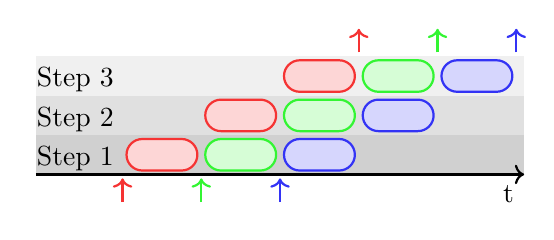
\begin{tikzpicture}[
	calc/.style ={rectangle,rounded corners=2mm, minimum width=.9cm, minimum height=.4cm,draw=#1,fill=#1!20,thick},
	step/.style ={rectangle, minimum width=6.2cm, minimum height=.5cm,fill=#1,thick}
	]
	
	\node at (1.5,0) [step={grey1}] {};
	\node at (1.5,.5) [step={grey2}] {};
	\node at (1.5,1) [step={grey3}] {};
	
	\node at (0,0) [calc={processred}] {};
	\node at (1,.5) [calc={processred}] {};
	\node at (1,0) [calc={processgreen}] {};
	\node at (2,1) [calc={processred}] {};
	\node at (2,.5) [calc={processgreen}] {};
	\node at (2,0) [calc={processblue}] {};
	\node at (3,1) [calc={processgreen}] {};
	\node at (3,.5) [calc={processblue}] {};
	\node at (4,1) [calc={processblue}] {};
	
	\draw (-.5,-.6) -- (-.5,-.3) [->,color=processred,thick];
	\draw (.5,-.6) -- (.5,-.3) [->,color=processgreen,thick];
	\draw (1.5,-.6) -- (1.5,-.3) [->,color=processblue,thick];
	\draw (2.5,1.3) -- (2.5,1.6) [->,color=processred,thick];
	\draw (3.5,1.3) -- (3.5,1.6) [->,color=processgreen,thick];
	\draw (4.5,1.3) -- (4.5,1.6) [->,color=processblue,thick];
	
	\draw (-1.6,-.25) -- (4.6,-.25) [->,,thick];
	\node at (4.4,-.5) {t};
	\node at (-1.1,-.05) {Step 1};
	\node at (-1.1,.45) {Step 2};
	\node at (-1.1,.95) {Step 3};
	
	\end{tikzpicture}
	\caption{Simple three-steps pipeline}
\end{wrapfigure}

The orchestration of the pipeline can be made with a clock that governs the sending of a step's outputs to the next one's inputs. The frequency of the clock will be determined by the longest step of the pipeline thus dividing the process in several simple steps can improve the throughput.\\


The introduction of a clock also makes interfacing with other processors easier. This is particularly relevant in the case of FPGAs that are often used in heterogeneous architecture.\\

The pipeline is built at the function level, which means that inputs and outputs of data-flow graphs are synchronized : inputs must provided at the same time and outputs will be ready simultaneously, instantly or after a given number of clock cycles.



\subsubsection{Introducing registers}
\indent


The introduction of pipeline stages  lies in the addition of registers through the computation process that will draw boundaries between the different parts of the calculation. Inferring the good places where to split the computation appears a complex job and the programmer should have a way to specify it to keep a precise control of the produce hardware configuration. 

\begin{wrapfigure}{r}{0.28\textwidth}
\vspace{-20pt}
\begin{lstlisting}[language=Whiley, frame=single, showlines=true]
function inc(bool a,
        int b) -> int:
    if a:
         b = b + 1
         skip
    return b
\end{lstlisting}
\end{wrapfigure}

\paragraph{The \whileyLine{skip} statement} \pindent


To study the impact and feasibility of this feature without modifying the language, the unused \whileyLine{skip} statement was reserved to indicate the introduction of stages on the computation of the current block of code.\\


\begin{wrapfigure}{r}{0.28\textwidth}
	\center
\vspace{-22pt}
	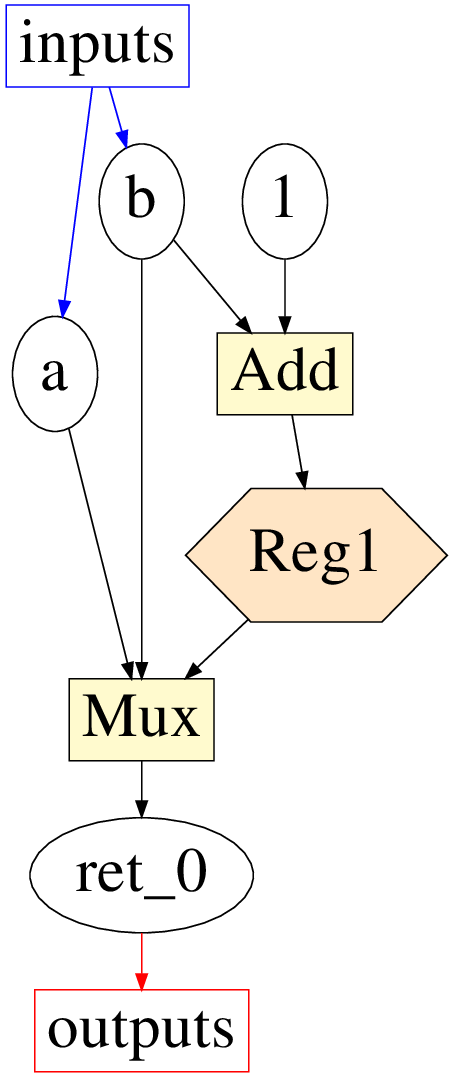
\includegraphics[scale=.22]{Reg_A.png}
	\caption{Resulting data-flow graph}
	%\vspace{-10pt}
	\label{fig:skip}
\end{wrapfigure}

When a \whileyLine{skip} statement is encountered, vertexes representing variables are transformed by adding to them a register. The compilation continues for ther remaining block's statements using these new vertexes. At the end of the block, unmodified variables are restored to their previous state.


\subsubsection{Synchronizing sources}
\indent

\begin{wrapfigure}{r}{0.3\textwidth}
	\vspace{-39pt}
	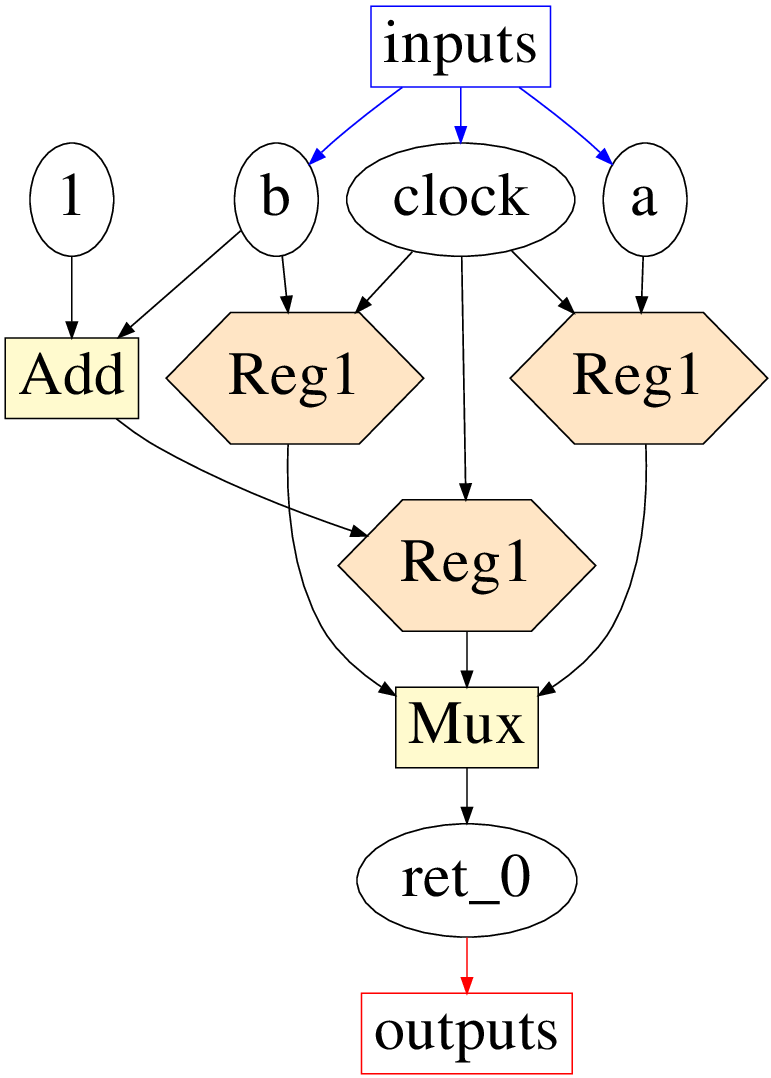
\includegraphics[scale=.23]{Reg_B.png}
	\caption{Synchronized data-flow graph}
\end{wrapfigure}

\paragraph{Modifying the language}\pindent

From the perspective of adapting the language to this specific compilation target, two ways of introducing registers could be considered~:

\begin{itemize}
	\item \textbf{A block boundary} : A specific keyword \code{split} or \code{stage} could be introduced to notify the splitting of a block into two parts.
	\item \textbf{A variable boundary} : Because splitting the whole block into two parts can be irrelevant (if one of the variables is known to be already the result of a several cycle computation), registers should be addable to precise variables. It can currently be achieved with the block boundary using a named block that modifies only the desired variable, but this work-around befuddles the resulting code.
\end{itemize}

These modifications could be gathered with a unique keyword that can be used either alone or with variables.


During the building of data-flow graphs, registers are only added where \whileyLine{skip} statements were encountered. The resulting graph may contain inconsistencies between sources: \autoref{fig:skip} shows the a vertex with two sources ready immediately whereas its last one needs one more cycle.\\

To ensure that the wanted result is computed, two constructions can be considered~:

\begin{itemize}
\item Keeping the same result as long as it may still be needed
\item Adding registers to delay early sources. 
\end{itemize}

The second option enable the pipeline to operate at its higher rate (one input per clock tick). It can however delay unnecessarily the result in the case of \code{mux} where the unselected option is ready after the selected one.


\subsection{Adding loops}
\indent

Loops are commonly used in software programming languages. However, HDL such as VHDL only allow loops with statically known number of iterations that can be unfold in the resulting design.

\subsubsection{General considerations on loops}\indent

A loop is a syntactical construction that enables a set of instructions (the body) to be successively executed a (possibly zero) number of time that depend on the value of a specific expression (the condition). Several facts need to be kept in mind to introduce their support.
\begin{itemize}
	\item Contrary to other statements, the length of the calculation may not be statically known, because the number of iteration is often dynamically determined.
	\item The same piece of code/circuit must be used several times in the computation of a single entry, owing to the fact that circuits/programs are spatially finite.
	\item This multiple use of the same circuit prevents to build a pipeline as it was previously described. The synchronization of vertexes' sources must be adapted to this new kind of unknown latency.
\end{itemize}

Loops where considered is the most general case, with no guarantee on their execution. When additional information is known, more relevant constructions can be set-up. A complete example (including simulation) is given in \hyperref[Ex]{appendix}. \\


\textbf{\textsl{Remark :}} Using unbound loops does not seem to be an appropriate design for hardware description. However, it may sometimes be relevant and adding their support made a comprehensive time analysis unavoidable, which improved greatly the processing of code without loops.


\subsubsection{Introducing loops in the data-flow graph} \indent

The conversion of \whileyLine {while} statements to data-flow graph vertexes is worth mentioning. A special \code {while} vertex is provided, whose sources are the variables that are used in the loop and which targets are new symbolic vertexes that represent the updated value of variables modified by the loop.\\

Additionally, this vertex contains two data-flow graphs : one for the body of the loop and an other for the computation of the condition.\\


\subsubsection{Adding state signals} \indent

During the time analysis, body and condition data-flow graphs of \code {while} vertexes are merged in the global graph, surrounded with additional logic.\\


In agreement with the computation model of VHDL, every part of the design will be evaluated at each cycle, whereas the computation needs several ones. A way to distinguish at runtime outputs that are meaningful from others (intermediate or irrelevant values) if thus needed. The addition of state signals gives a way to represent the progress of the computation.\\


A simple approach uses only two state signals : a \textit{Start} input signal that is activated when entries are sent, and a \textit{Done} output one that indicates when circuit's outputs are ready.

	
	\begin{figure}[h]
		\center
		\begin{circuitikz}[-,terminal/.style={
				% The shape:
				rounded rectangle,
				minimum size=1.6mm,
				% The rest
				thick,draw=black}]
			
			\draw (8.2,7) node[Reg] (RegS) {};
			\draw (8.2,3) node[Reg] (RegD) {};
			
			\draw (-1.5,3) node (inputs) {};
			\draw (12.5,3) node (outputs) {};
			
			\draw (0.5,3) node (step) {};
			\draw (step)+(-.5,0) node (stepR) {};
			
			\draw 
				(5.5,5) node[BlockCB,align=center] (While) {\Large Condition \\ \Large \& \\ \Large Body}
				
				(While.out data) -- ++(1.1,0) |- (RegD.east)
			;	
			\draw (While.in start -| step) node[or port] (OrS) {};
			\draw (OrS)+(-.55,0) node {\textbf{Or}};
			\draw (While.in data -| stepR) node[muxT] (MuxD) {};
			
			\draw 
				(OrS.in 2 -| inputs) node[terminal] (S) {Start}
				
				(OrS.out) -- ++(.2,0) |- (While.in start)
				
				(S.east) -| (OrS.in 2)
				(RegS.west) -| (OrS.in 1)
			;
			\draw 
				(MuxD.in true -| inputs) node[terminal] (D) {Data}
				
				(MuxD.out) -- ++(.6,0) |- (While.in data)
				
				(S.east)+(0.1,0) |- (MuxD.in cond)
				(D.east) -| (MuxD.in true)
				(RegD.west)   -| (MuxD.in false)
			;
			
			\draw 
				(10.1,6) node[and port] (AndS) {}
				(While.out done) -- ++(.2,0) |- (AndS.in 1)
				(While.out test) -- ++(.6,0) |- (AndS.in 2)
				(AndS.out) |- (RegS.east)
			;	
			\draw (AndS)+(-.65,0) node {\textbf{And}};
			
			\draw
				(1.4,5.3) node[muxT,red] (DataS) {}
				(MuxD.out) |- (DataS.in true)
				(OrS.out) -| (DataS.in cond)
			;
			\draw
				(DataS)+(1,-0.75) node[Reg,red] (RegDa) {}
				(RegDa.west) -| (DataS.in false) [red]
			;
			
			
			\draw 
				(9.5,4.55) node[not port] (Not) {}
				(While.out test) -- ++(.6,0) |- (Not.in)
			;	
			\draw (Not)+(-.15,0) node {\textbf{Not}};
			
			\draw 
				(11.7,5) node[and port] (AndNS) {}
				(While.out done) -- ++(.2,0) |- (AndNS.in 1)
				(Not.out) |- (AndNS.in 2)
			;	
			\draw (AndNS)+(-.65,0) node {\textbf{And}};
			\draw 
				(AndNS.out -| outputs) node[terminal] (Done) {Done}
				(AndNS.out) -- (Done.west)
			;
			\draw 
				(12.5,2.3) node[terminal] (Res) {Data}
				(DataS.out)  -- ++(1.3,0) |- (Res.west)
			;
			
			\draw
				(DataS.out) -- ++(1.3,0) |- (RegDa.east) [red]
			;
			
			
		\end{circuitikz}
		\caption[]{Additional logic around loops (American circuit diagram  style\footnotemark)}
		\label{Dloops}
	\end{figure}
	

\autoref{Dloops} details the additional logic built around loop's body and condition in a simple case where they are supposed to be ready at the same time.  This diagram shows that an extra iteration is computed, that is dropped if not necessary. The results of the previous iteration (or the inputs) are stored in a buffer waiting for the condition value to be ready.






\footnotetext{Node shapes convention can be found \href{https://en.wikipedia.org/wiki/Logic_gate}{here}}


\begin{wrapfigure}[30]{r}{.38\textwidth}
%\vspace{-15pt}
\center
	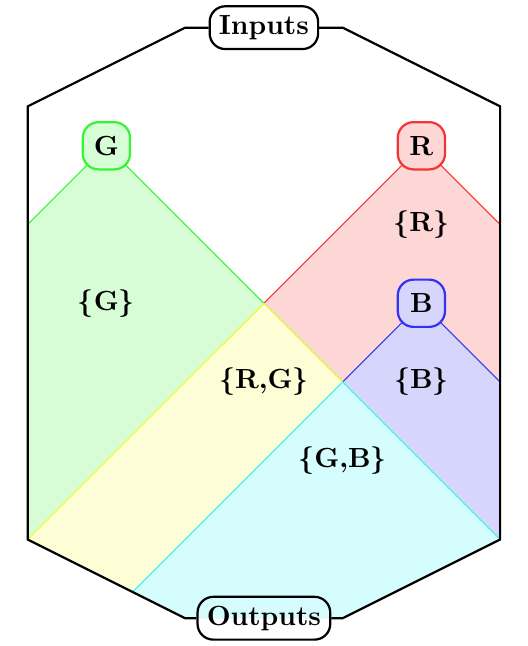
\begin{tikzpicture}[
		while/.style ={rectangle,rounded corners=2mm, minimum width=.6cm, minimum height=.6cm,draw=#1,fill=#1!20, thick,align=center}	
	]
	
	\def\border{(2,-1) -- (0,0) -- (0,5.5) -- (2,6.5) -- (4,6.5) -- (6,5.5) -- (6,0) -- (4,-1) -- cycle}
	\def\reversed{(-10,10) -- (-10,-10) -- (10,-10) -- (10,10) -- (-10,10)}
		\path[name path=border] \border;
	

\begin{pgfinterruptboundingbox}
	\foreach \n/\c/\p in {{R/processred/(5,5)},{G/processgreen/(1,5)},{B/processblue/(5,3)}}{
		\begin{scope} % red + green = yellow
			\clip \p -- +(8,-8) -- +(-8,-8) -- cycle;
			\draw [fill=\c!20,draw=none] \border;
		\end{scope}
		\path[name path=lg] \p -- ++(-8,-8);
		\path[name path=rg] \p -- ++(8,-8);
		\path [name intersections={of=border and lg,by=liW\n}];
		\path [name intersections={of=border and rg,by=riW\n}];
		\draw [-, \c]
			\p -- (liW\n)
			\p -- (riW\n)
		;
		\node at \p [while={\c}] (W\n) {};
		\node at \p {\textbf{\n}};
}

	\begin{scope}
		\clip (WR) -- ++(-8,-8) -- +(16,0) -- (WR)-- cycle;
		\clip (WG) -- ++(-8,-8) -- +(16,0) -- (WG)-- cycle;
		\draw[-,fill=processyellow!20,draw=none] \border;
	\end{scope}	
	\begin{scope}
		\clip \border;
		\clip (WG) -- ++(-8,-8) -- +(16,0) -- (WG)-- cycle;
		\draw[-,draw=processyellow] (WR) -- +(-8,-8);
	\end{scope}	
	\begin{scope}
		\clip \border;
		\clip (WR) -- ++(-8,-8) -- +(16,0) -- (WR)-- cycle;
		\draw[-,draw=processyellow] (WG) -- +(8,-8);
	\end{scope}	
	\begin{scope}
		\clip (WG) -- ++(-8,-8) -- +(16,0) -- (WG)-- cycle;
		\clip (WB) -- ++(-8,-8) -- +(16,0) -- (WB)-- cycle;
		\draw[-,fill=processcyan!20,draw=none] \border;
	\end{scope}	
	\begin{scope}
		\clip \border;
		\clip (WG) -- ++(-8,-8) -- +(16,0) -- (WG)-- cycle;
		\draw[-,draw=processcyan] (WB) -- +(-8,-8);
	\end{scope}	
	\begin{scope}
		\clip \border;
		\clip (WB) -- ++(-8,-8) -- +(16,0) -- (WB)-- cycle;
		\draw[-,draw=processcyan] (WG) -- +(8,-8);
	\end{scope}	
	
	\begin{scope}
		\node at (3,6.5) [rectangle,rounded corners=2mm,thick,draw=black] (In) {\textbf{Inputs}};
		\node at (3,-1) [rectangle,rounded corners=2mm,thick,draw=black] (Out) {\textbf{Outputs}};
		\clip \reversed -- (In.north east) rectangle (In.south west) ;
		\clip \reversed -- (Out.north east) rectangle (Out.south west) ;
		\draw [-, thick] \border;
	\end{scope}
\end{pgfinterruptboundingbox}
	
		\node at (1,3) {\textbf{\{G\}}};
		\node at (5,4) {\textbf{\{R\}}};
		\node at (5,2) {\textbf{\{B\}}};
		\node at (3,2) {\textbf{\{R,G\}}};
		\node at (4,1) {\textbf{\{G,B\}}};
	
	\end{tikzpicture}
	\caption{Abstract representation of a data-flow graph with 3 inner seeds and their zone of influence}
	\label{LSync}
\end{wrapfigure}

\subsubsection{Synchronizing sources} \indent

The synchronization of data that can be ready an arbitrary time after the beginning of calculation necessitates the use of buffers. The red part of \autoref{Dloops} circuit shows a simple buffer that updates its value regarding a storing signal. \\


A first approach to sources synchronization consists in adding a \textit{delay} information (number of cycles needed or special unknown value) to vertexes that handles the length of computation from inputs to it. Buffers are then added between a vertex and its sources if one of them has an unknown delays (early sources will "wait" in buffers until they are all ready). This leads to an over used of such components (for example if sources come from the same while construction) that should be avoided. \\


A more relevant study of delays can save a lot of these useless buffers : \textit{calculation seeds} are added to represent circuit places where the result can be ready at an arbitrary time after the calculation of sources and vertexes are decorated with the set of \textit{seeds} from which they are delayed by a known number of cycles. These seeds are either a special input seed or inner seeds that correspond to vertexes with an unknown latency (while nodes or functions call with an unknown latency). The data-flow graph is thus divided into parts sharing the same set of seeds, and buffers are only needed when sources are in different zones.



\subsubsection{Improving concurrency} \indent

The introduction of loops greatly reduces the possible concurrency : a new computation cannot be start as long as a loop is still running because it could be still unfinished when new data will come to it. Some enhancements can nevertheless be achieved.




\definecolor {cycle0}{hsb}{0,1,1}
\definecolor {cycle0.5}{hsb}{.03,1,1}
\definecolor {cycle1}{hsb}{.06,1,1}
\definecolor {cycle1.5}{hsb}{.09,1,1}
\definecolor {cycle2}{hsb}{.12,1,1}
\definecolor {cycle2.5}{hsb}{.15,1,1}
\definecolor {cycle3}{hsb}{.18,1,1}
\definecolor {cycle3.5}{hsb}{.21,1,1}
\definecolor {cycle4}{hsb}{.24,1,1}


\definecolor {cond1}{hsb}{.8,0,.8}
\definecolor {cond2}{hsb}{.8,0,.85}
\definecolor {cond3}{hsb}{.8,0,.9}
\definecolor {cond4}{hsb}{.8,0,.95}
\definecolor {sep}{hsb}{.6,.6,.6}

\begin{wrapfigure}[17]{r}{.6\textwidth}
	\vspace{-30pt}
	\center
	\begin{tikzpicture}[
	body/.style 2 args={shading = axis, shading angle = 0, rectangle,rounded corners=2mm, minimum width=.9cm, minimum height=.4cm,draw=#1,left color=#1!20, right color=#2!20, draw=none,horizontal shaded border=#1 and #2},
	cond/.style ={rectangle,rounded corners=2mm, minimum width=.9cm, minimum height=.4cm,draw=#1,fill=#1!20, thick,text height=.2cm,align=center},
	buff/.style ={rectangle,rounded corners=2mm, minimum width=1.9cm, minimum height=.4cm,draw=#1,fill=#1!20, thick,text height=.2cm,align=center},
	step/.style ={rectangle, minimum width=9.6cm, minimum height=.5cm,fill=#1,draw=none}
	]
	
	\node at (2.7,0) [step={cond1}] {};
	\node at (2.7,.5) [step={cond4}] {};
	\node at (2.7,1) [step={cond1}] {};
	\node at (2.7,1.5) [step={cond2}] {};
	\node at (2.7,2) [step={cond3}] {};
	\node at (2.7,2.5) [step={cond4}] {};
	\node at (2.7,3) [step={cond1}] {};
	\node at (2.7,3.5) [step={cond4}] {};
	
	\node at (0,1) [cond={cycle0}] {};
	\node at (0,0) [body={cycle0}{cycle0.5}] {};
	\node at (.5,3) [buff={cycle0}] {};
	\node at (1,1.5) [cond={cycle0}] {};
	\node at (1,.5) [body={cycle0.5}{cycle1}] {};
	\node at (2,2) [cond={cycle0}] {};
	\node at (2,1) [cond={cycle1}] {};
	\node at (2,0) [body={cycle1}{cycle1.5}] {};
	\node at (2.5,3) [buff={cycle1}] {};
	\node at (2.5,3.5) [buff={cycle0}] {};
	\node at (3,2.5) [cond={cycle0}] {\small{0}};
	\node at (3,1.5) [cond={cycle1}] {};
	\node at (3,.5) [body={cycle1.5}{cycle2}] {};
	\node at (4,2) [cond={cycle1}] {};
	\node at (4,1) [cond={cycle2}] {};
	\node at (4,0) [body={cycle2}{cycle2.5}] {};
	\node at (4.5,3) [buff={cycle2}] {};
	\node at (4.5,3.5) [buff={cycle1}] {};
	\node at (5,2.5) [cond={cycle1}] {\small{0}};
	\node at (5,1.5) [cond={cycle2}] {};
	\node at (5,.5) [body={cycle2.5}{cycle3}] {};
	\node at (6,2) [cond={cycle2}] {};
	\node at (6,1) [cond={cycle3}] {};
	\node at (6,0) [body={cycle3}{cycle3.5}] {};
	\node at (6.5,3) [buff={cycle3}] {};
	\node at (6.5,3.5) [buff={cycle2}] {};
	\node at (7,2.5) [cond={cycle2}] {\small{1}};
	\node at (7,1.5) [cond={cycle3}] {};
	\node at (7,.5) [body={cycle3.5}{cycle4}] {};
	
	\draw (-.5,-.6) -- (-.5,-.3) [->,color=cycle0,thick];
	\draw (7.5,3.75) -- (7.5,4.05) [->,color=cycle2,thick];

	
	\draw (-2.1,-.25) -- (7.6,-.25) [->,thick];
	\draw (-2.1,.75) -- (7.5,.75) [-,thick, sep];
	\draw (-2.1,2.75) -- (7.5,2.75) [-,thick, sep];
	
	\node at (7.4,-.5) {t};
	\node at (-1.1,-.05) {Step 1};
	\node at (-1.1,.45) {Step 2};
	\node at (-1.1,.95) {Step 1};
	\node at (-1.1,1.45) {Step 2};
	\node at (-1.1,1.95) {Step 3};
	\node at (-1.1,2.45) {Step 4};
	\node at (-1.1,2.95) {Reg 1};
	\node at (-1.1,3.45) {Reg 2};
	
	\node at (-1.85,.25) [rotate=90] {\textbf{Body}};
	\node at (-1.85,1.75) [rotate=90] {\textbf{Condition}};
	\node at (-1.85,3.25) [rotate=90] {\textbf{Sync}};
	
	\end{tikzpicture}
	\caption{Optimized loop construction in the case of a 2-cycles long body and a 4-cycles long condition}
\end{wrapfigure}

\paragraph{Improving loop construction}\pindent

Synchronizing body and condition of loops is unnecessary : the computation can stop as soon as the result of the condition is ready and false. However, it necessary to wait for the body to complete before starting to evaluate the next condition's value.


\paragraph{Defining  concurrency}\pindent

Without further knowledge, a decent concurrency/space trade-off consists in setting the maximum number of values that can be processed at the same time. Fixed-size buffers and then needed before loops to ensure smth.
 
\subsection{Future work} \indent

This study has set up some bases of compilation toward FPGAs, but several subjects could be further studied :

\begin{itemize}
	\item \textbf{Targeting net-list} : To avoid as much as possible the dependency toward proprietary tools, net-lists could be produced instead of VHDL.
	\item \textbf{Type representation optimization} : A deeper analysis of types could lead to more compact representation of typed values, with less redundancy. 
	\item \textbf{Data-flow graph optimization} : Several simplification of data-flow graphs would Optimization on the data-flow graph could improve the generated code briefness.
	\item \textbf{Using constraint informations} : Analysing constraints on types would enable to adjust more sharply the representation to the possible values.
	\item \textbf{Adding bounds on loops} : Further information on loop execution (bounds on the number of iterations) that should be checkable by the theorem prover lead to a very interesting on the building of an optimized pipeline.
	\item \textbf{Inlining relevant function} : In order to avoid synchronization of inputs and outputs, the data-flow graph of certain called functions could be inserted in the caller's one.
	\item Improving the language support (array, complex operations, part of references)
\end{itemize}
 
\section*{Conclusion}\indent
\addcontentsline{toc}{section}{Conclusion}

 

Hardware configurations cannot be designed the way software programs are. The addition of specific language constructions is required to turn Whiley into an effective high-level HDL. Whereas some high-level features like flow-typing are well-suited for hardware compilation,  the support of other software programming language constructs like loops should be carefully considered (the compiler could issue warnings about them), mainly because they introduce new signals that are not usable in the high-level description (impossible to read the \textit{done} flag in Whiley sources to synchronize another part). \\

It may be relevant to introduce such structures in the high-level language, by providing objects that exhibit their internal construction to ensure the finest control over the resulting design.
 
 
 \newpage
 \bibliographystyle{alpha}
 \bibliography{References}
\newpage
\section*{Annex : A working example}\indent
\label{Ex}
\addcontentsline{toc}{section}{Annex : A working example}

A naive implementation of Euclidean division of positive integers was chosen to enlighten the main features of the compiler.

\newbox\wcode
\begin{lrbox}{\wcode}
\begin{minipage}[t]{.45\textwidth}
\begin{lstlisting}[language=Whiley, frame=single, showlines=true, numbers=left]
type Result is {int q, int r}

function div(int a, int b) 
    -> Result|null:
  if b==0:
    return null
  Result d = {q:0,r:a}
  while d.r >= b:
    d.q = d.q + 1
    d.r = d.r - b
  return d

function main(int a, int b) 
    -> (int q,int r):
  Result|null d = div(a,b)
  if d is Result:
    return d.q,d.r
  return 0,0
\end{lstlisting}
\end{minipage}
\end{lrbox}

\begin{figure}[H]
\vspace{-10pt}
\centering
\subfloat[Division implementation]{\adjustbox{valign=b}{\usebox\wcode}}
\quad \subfloat[Synchronized data-flow graph of \lstinline{main} function]{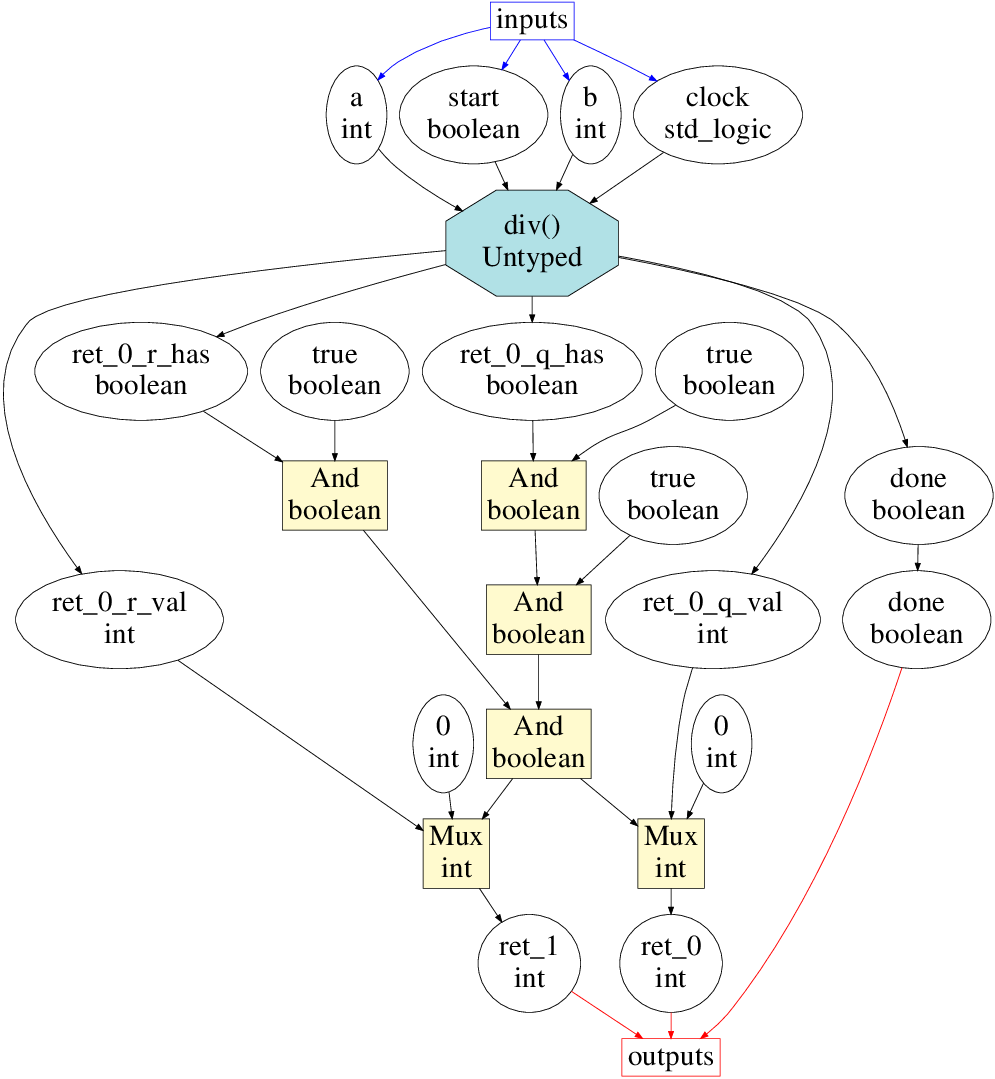
\includegraphics[width=.48\textwidth]{MainSync.png}}

\subfloat[Screen-shot of the simulator. (Colours were modified to improve readability) Computations start at the first clock rising edge after the change of a entry]{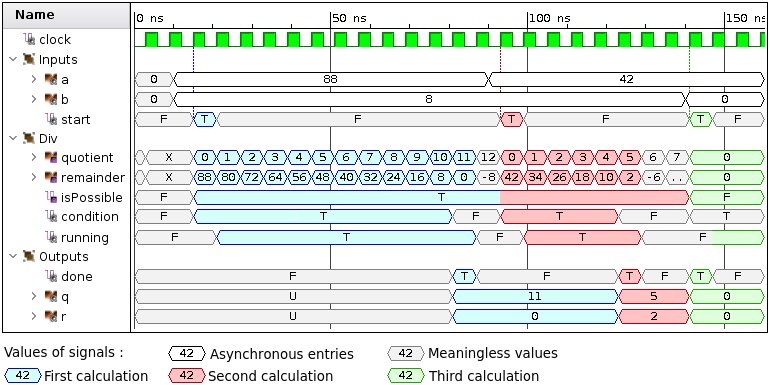
\includegraphics[width=\textwidth]{While_Sim.png}}
\caption {Example of assignment}
\end{figure}

The \whileyLine {div} function leads to a complex data-flow graph. The one of \whileyLine {main} function highlights how function invocation is represented and how flow typing operation \whileyLine{is} operator is converted (\code {and} nodes).

The generated VHDL code is introduced in a testing project that defines the values of inputs through time. Its simulation shows that expected values a actually computed and that it requires a variable time (delay between \textit{start} and \textit{done} \code {True} values).


\end{document}